%----------------------------------------------------------------------------
\chapter{\SystemDesign}
%----------------------------------------------------------------------------
\section{Követelmények}
%----------------------------------------------------------------------------
Az új rendszer tervezésekor a következő szempontokat kellett szem előtt tartanom:
\begin{itemize}
	\item Teljesen digitális megoldás kialakítása.
	\item Redundáns rendszer kialakítása biztosítva a folyamatos működést.
	\item Rugalmas felépítés, amely lehetővé teszi a könnyű alkalmazkodást változó körülményekhez.
	\item Könnyen bővíthető struktúra kialakítása a jövőbeli igényekhez való gyors reagálás érdekében.
	\item Magasabb hangminőség és hangnyomás elérése a korábbi rendszerrel összehasonlítva.
	\item Jobb lefedettség és egyenletes hangvisszaadás biztosítása a közönség területén.
	\item A piacon lévő termékekhez képest viszonylag költséghatékony megoldás kidolgozása.
	\item Legyen hosszú távon egy kompetitív és korszerű rendszer.
	\item Megbízható és kiforrott technológiára épüljön.
\end{itemize}
%----------------------------------------------------------------------------
\section{Rendszerterv}
%----------------------------------------------------------------------------
A cég alapítása óta Martin Audio termékeket használ, a régi W8LM rendszerrel nagyon elégedettek voltunk, 
ebből kifolyólag a választás márka szempontjából nem is volt kérdéses. A Martin új rendszerei a Wavefront Precision sorozat szériás
végfokai pedig a Dante hálózatot használja a digitális hangátvitelhez.
Ebből kifolyólag a választás a Dante protokollra esett, így a szakdolgozatomban 
megtervezésre kerülő hangrendszer lelke ez a protokoll lesz.
Hangládák szempontjából a Martin Audio Wavefront Precision szériás termékein belül kétfajta rendszerre is esett választás.
Ezekről a későbbiekben részletesen lesz szó.
Mivel teljes mértékben digitális rendszert elérése volt a cél, ezért a Dante modullal
rendelkező Martin Audio iKON iK42 és iK81 végfokok tökéletesen illeszkedtek a rendszerbe.
Mindkét végfok csúcskategóriás teljesítményt és hangminőséget nyújt, és a D kategóriás
erősítőknek köszönhetően rendkívül kis helyet foglalnak el a rack-ben miközben kiváló hatásfok
mellett képesek nagy teljesítményt leadni. A két erősítő között két fundamentális különbség van,
az iK42 négy kimeneti csatornával rendelkezik, 20.000 W teljesítmény leadása mellett. 
Ezzel szemben az iK81 nyolc kimeneti csatornával rendelkezik, 10.000 W teljesítménnyel. \cite{IKONAMPUSEGUIDE}
A végfokokat a Dante hálózaton keresztül fogjuk jellel ellátni, így a hagyományos analóg XLR, vagy AES kábelezés helyett
két CAT5E kábellel (a redundancia miatt) tudjuk a végfokokat a hálózatra kötni. 
%----------------------------------------------------------------------------
\begin{figure}[H]
    \centering
    \begin{minipage}{0.45\textwidth}
        \centering
        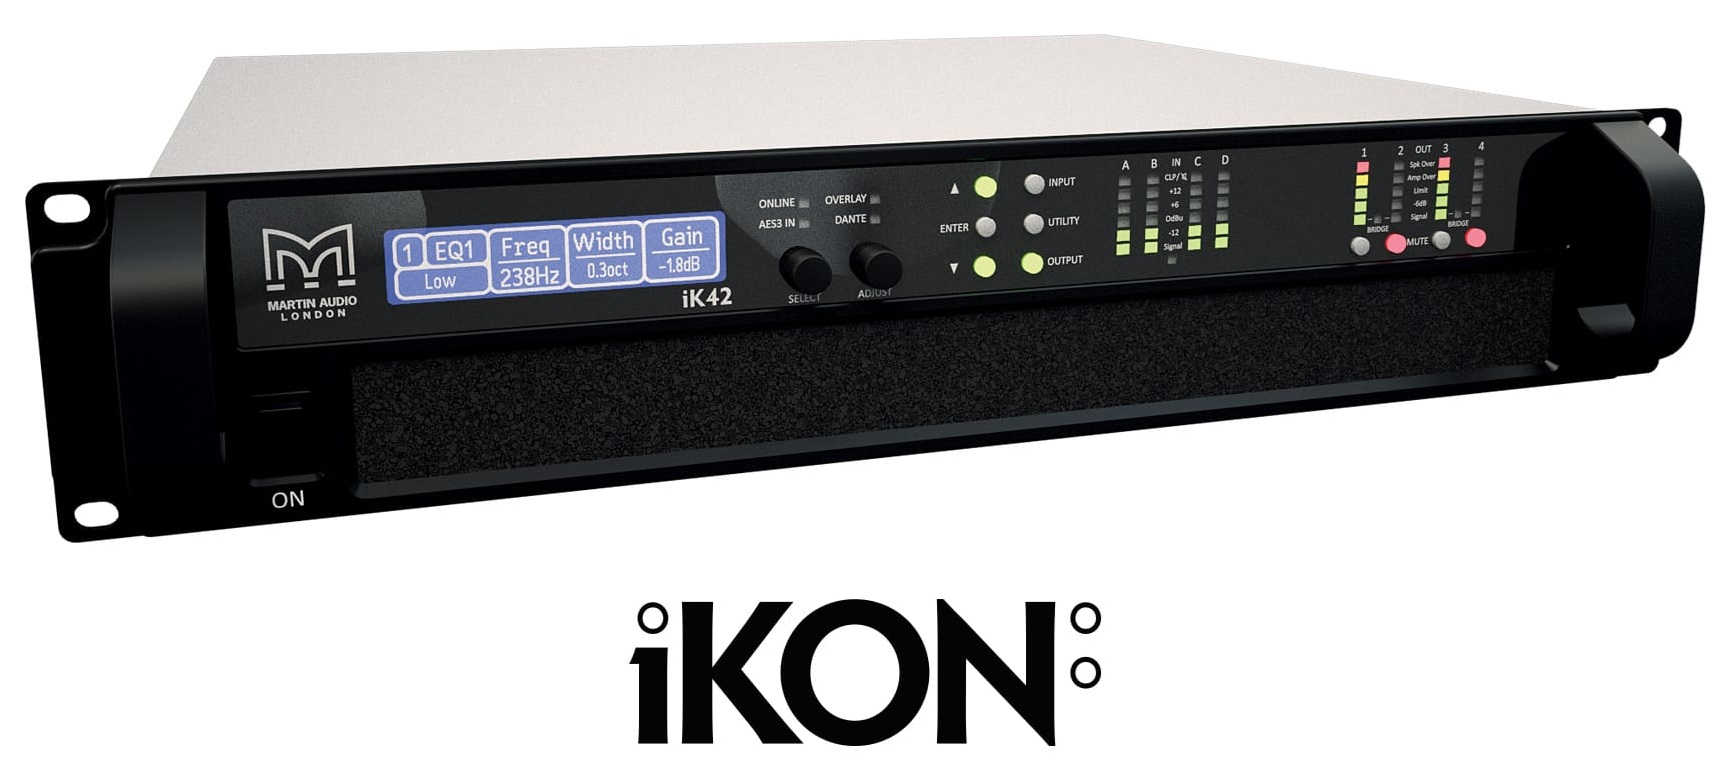
\includegraphics[width=\linewidth, keepaspectratio]{figures/ikon_ik42.jpg}
        \caption{Martin Audio iK42 végfok}\label{fig:ikon_ik42}
    \end{minipage}\hfill
    \begin{minipage}{0.45\textwidth}
        \centering
        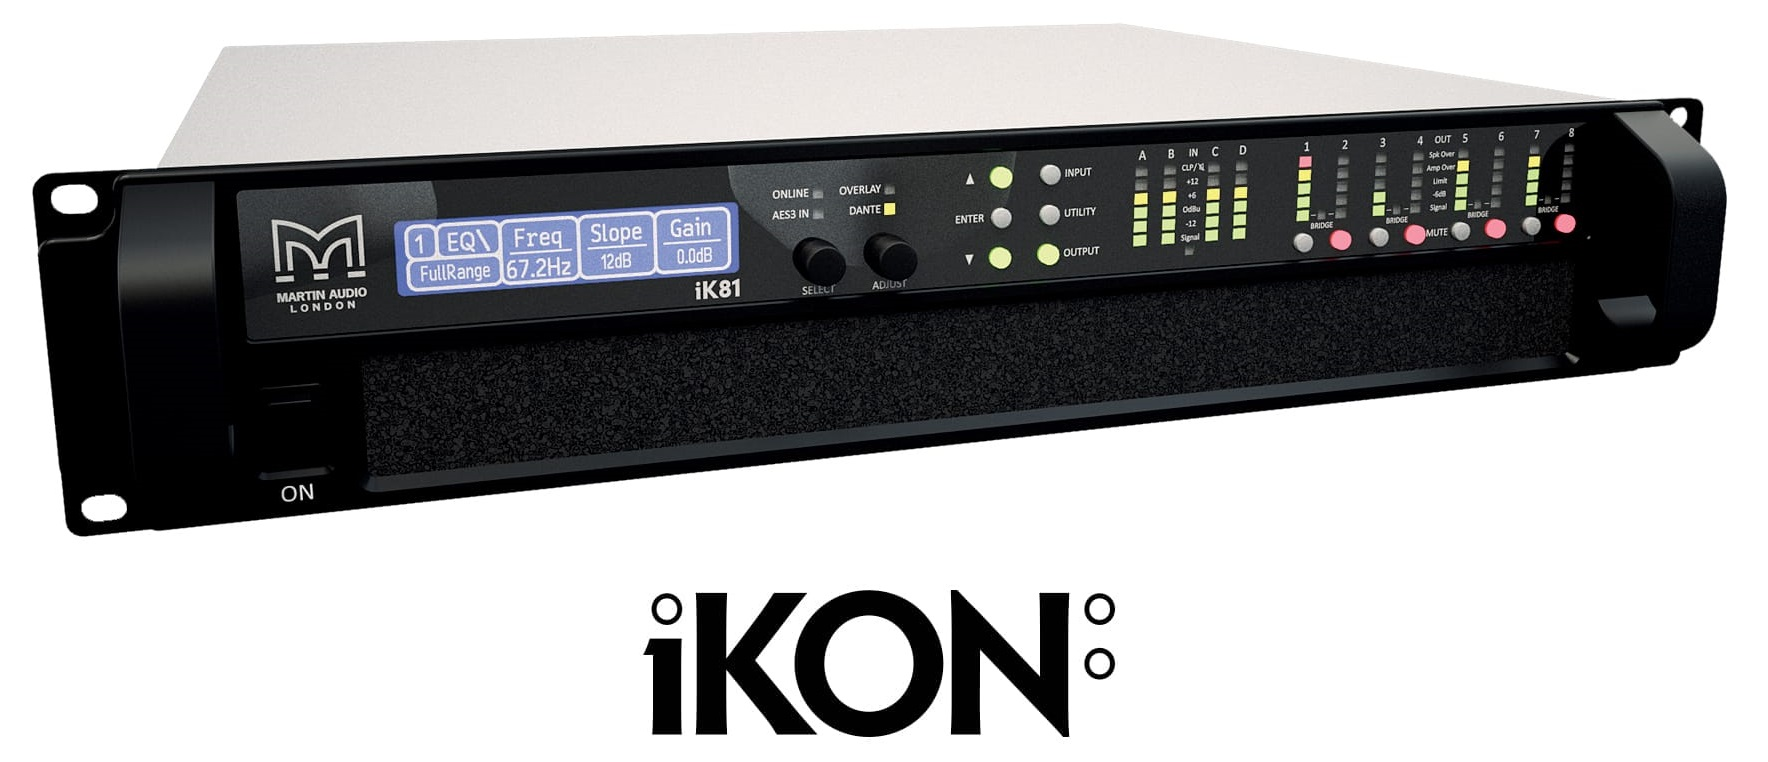
\includegraphics[width=\linewidth, keepaspectratio]{figures/ikon_ik81.jpg}
        \caption{Martin Audio iK81 végfok}\label{fig:ikon_ik81}
    \end{minipage}
\end{figure}
%----------------------------------------------------------------------------
A végfokrendszer fő vezérlő protokollja miatt szükség lesz még egy CAT5E alapú
összeköttetésre, ami az egyes végfokokat köti össze egy hálózatba a switcheken keresztül. (VU-NET protokoll)
Minden egyes végfokrackben két MikroTik 24 portos switch lesz. 
Ezekre az eszközökre készítettem egy unified konfigurációt, amely minden olyan felesleges biztonsági
beállítást kikapcsol, amelyekre egy normál internetes hálózatban szükség lenne, de egy zárt hálózatban ahol kizárólag
a Dante eszközök kommunikálnak egymással, ezek a beállítások csak felesleges terhelést jelentenének a hálózaton.
Valamint amennyiben még több eszközt szeretnénk a hálózatra kötni, akkor a switchek gyorsan üzembe helyezhetőek,
mivel a konfiguráció már előre elkészítve, csak fel kell tölteni a beállításokat, valamint firmware-t egyeztetni.
%----------------------------------------------------------------------------
Az egyik switch a Dante elsődleges hálózatát fogja kizárólag kezelni.
A másik switch a Dante másodlagos hálózatát, és a VU-NET hálózatot fogja kezelni.
Ez a két alhálózat VLAN szegmensekbe lesz elkülönítve, hogy a hálózat biztosan stabil legyen, ne fordulhassanak elő csomagütközések.
A rendszer kábelezése egyedileg készített Neutrik EtherCon csatlakozóval ellátott CAT5E és CAT6A kábelekből fog állni.
A kábelek készítésekor a T568B szabvány szerinti kábelrendezést alkalmazom, mivel a T568B jobb átviteli
teljesítményt és interferencia védelmet nyújt a hosszú távú használat során.
Nem szükséges a T568A szabvány által nyújtott plusz kompatibilitás a régi hálózatokkal, mivel egy teljesen új 
modern hálózatot fogunk kiépíteni. 
A csatlakozók felhelyezésekor a szabványnak megfelelően járok el, milliméterre pontosan, hogy a kábelek
a lehető legjobb minőségűek legyenek. Ez a CAT6A kábeleknél különösen fontos, mivel a CAT6A kábelek
még nagyobb frekvencia tartományban képesek adatokat továbbítani, mint a CAT5E kábelek,
ezért jobban érzékenyek a külső interferenciákra.
A végfokokból egy egyedi patch panel segítségével vezetjük ki a végpontokat, hogy ne az eszköz saját csatlakozóját
degradáljuk a sokszori csatlakoztatás során, hanem a patch panelen lévőt, melyet amennyiben szükséges könnyen cserélhetünk.
Valamint az eszközön lévő csatlakozó egy szabványos RJ45 csatlakozó nem pedig egy Neutrik EtherCon csatlakozó.
Számunkra ez is fontos, mivel a Neutrik csatlakozók strapabíróbbak, és a kábelvégek is jobban védettek a sérülésektől,
és nehezen vagy egyáltalán nem lehet véletlenül kihúzni a csatlakozót a helyéről.
%----------------------------------------------------------------------------
Az egyes végfokrackek összeköttetésért egy hibrid kábel lesz a felelős, amelyben négy darab CAT6A kábel van,
mindegyik véget külön színkóddal látjuk el, annak érdekében, hogy gyorsan és egyértelműen tudjuk azonosítani a kábeleket,
amikor egy adott helyszínen építjük össze a felszerelést, akár sok-sok óra munka után fáradtan.
A zöld szín jelzi majd a Dante elsődleges hálózatot, a kék szín a Dante másodlagos hálózatot, a piros szín a VU-NET hálózatot,
a fekete vég pedig egy tartalék kábel lesz, amennyiben valamelyik kábel megsérülne, vagy egyéb okból nem működne.
Mivel az előbbiekben már említett 24 portos switcheket használjuk, ezért ha vendég vagy bérelt eszközöket szeretnénk a hálózatra kötni,
akkor a switchekben található portokból ki tudjuk választani a megfelelő VLAN szegmenst, és a hozzá tartozó portokat,
így szabványos RJ45 csatlakozóval ellátott kábeleket Ethercon nélkül is tudunk használni.
Mindegyik rack hátuljában található még egy Wi-Fi router is, amely általában a VU-NET hálózatra kapcsolódik,
így a teljes rendszer vezérlése Wi-Fi-n keresztül is lehetséges lesz.
A Dante patch-et általában vezetékes módon fogjuk elkészíteni, de amennyiben készülékünk nem rendelkezik RJ45 csatlakozóval,
ami sajnos manapság egyre gyakoribb, akkor a Wi-Fi router segítségével is tudjuk konfigurálni a shared mode bekapcsolásával 
a Dante vezérlőben.
Az FOH (Front of House) pultot szintén egy hibrid kábel fogja összekötni a végfokrackekkel, amelyben viszont
már csak két darab CAT5E, két darab DMX és egy darab 230V-os tápkábel lesz. Ezzel a megoldással időt és helyet spórolunk,
az építésnél, mivel nem kell külön-külön vezetékeket kihúzni, elég egy kábelt, amelyben minden szükséges vezeték benne van.
%----------------------------------------------------------------------------
Tehát összefoglalva három egymástól teljesen elkülönített hálózatot fogunk kiépíteni a rendszer kiszolgálására,
a Dante elsődleges és másodlagos hálózatot, valamint a VU-NET hálózatot.

%----------------------------------------------------------------------------
\begin{figure}[H]
	\centering
	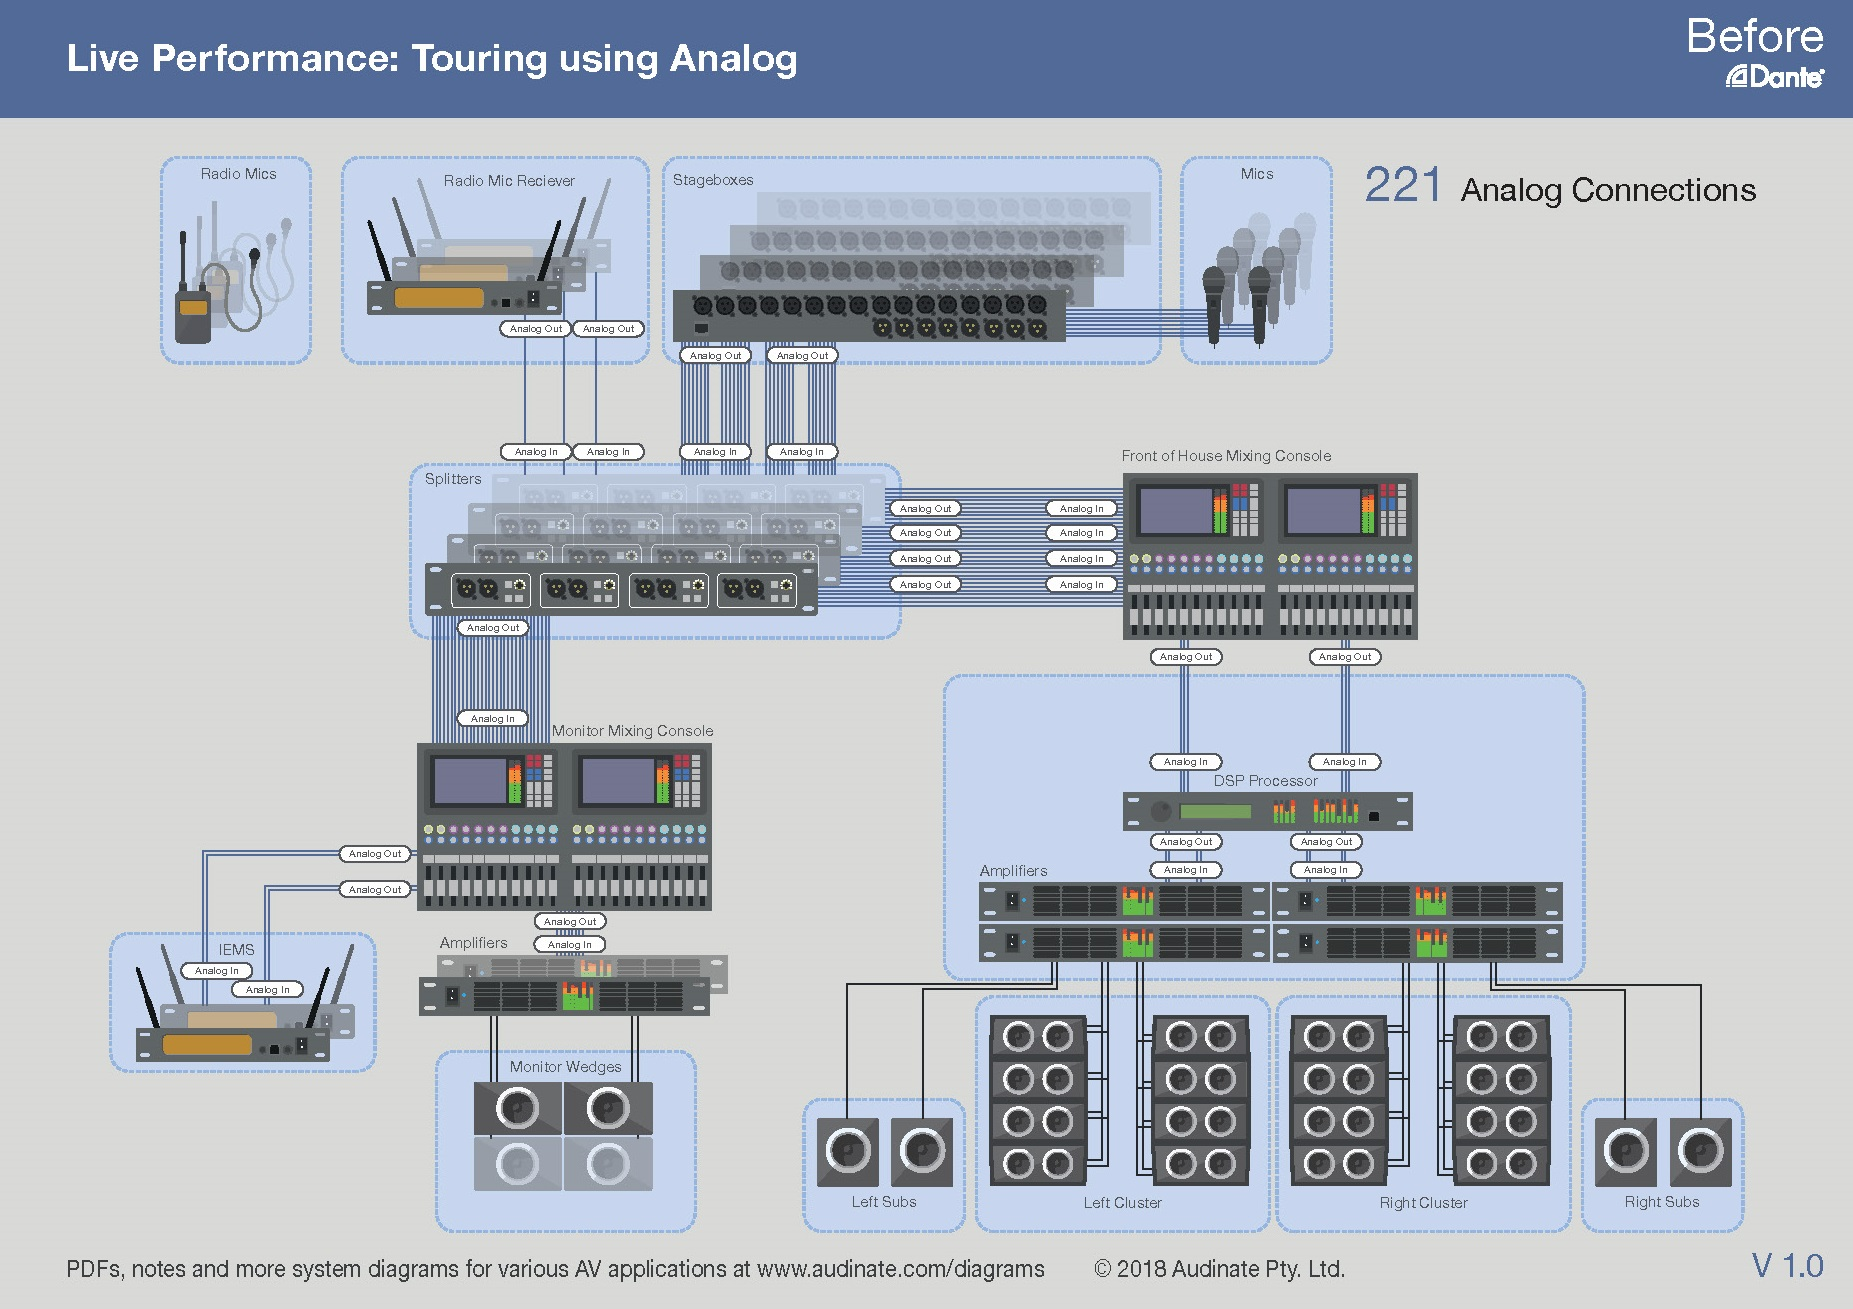
\includegraphics[width=\linewidth, keepaspectratio]{figures/live-analog.jpg}
	\caption{Példa hagyományos analóg kábelezésre \cite{APPLICATIONDIAGRAMSFORDANTESYSTEMS}}\label{fig:live-analog}
\end{figure}
%----------------------------------------------------------------------------
\begin{figure}[H]
	\centering
	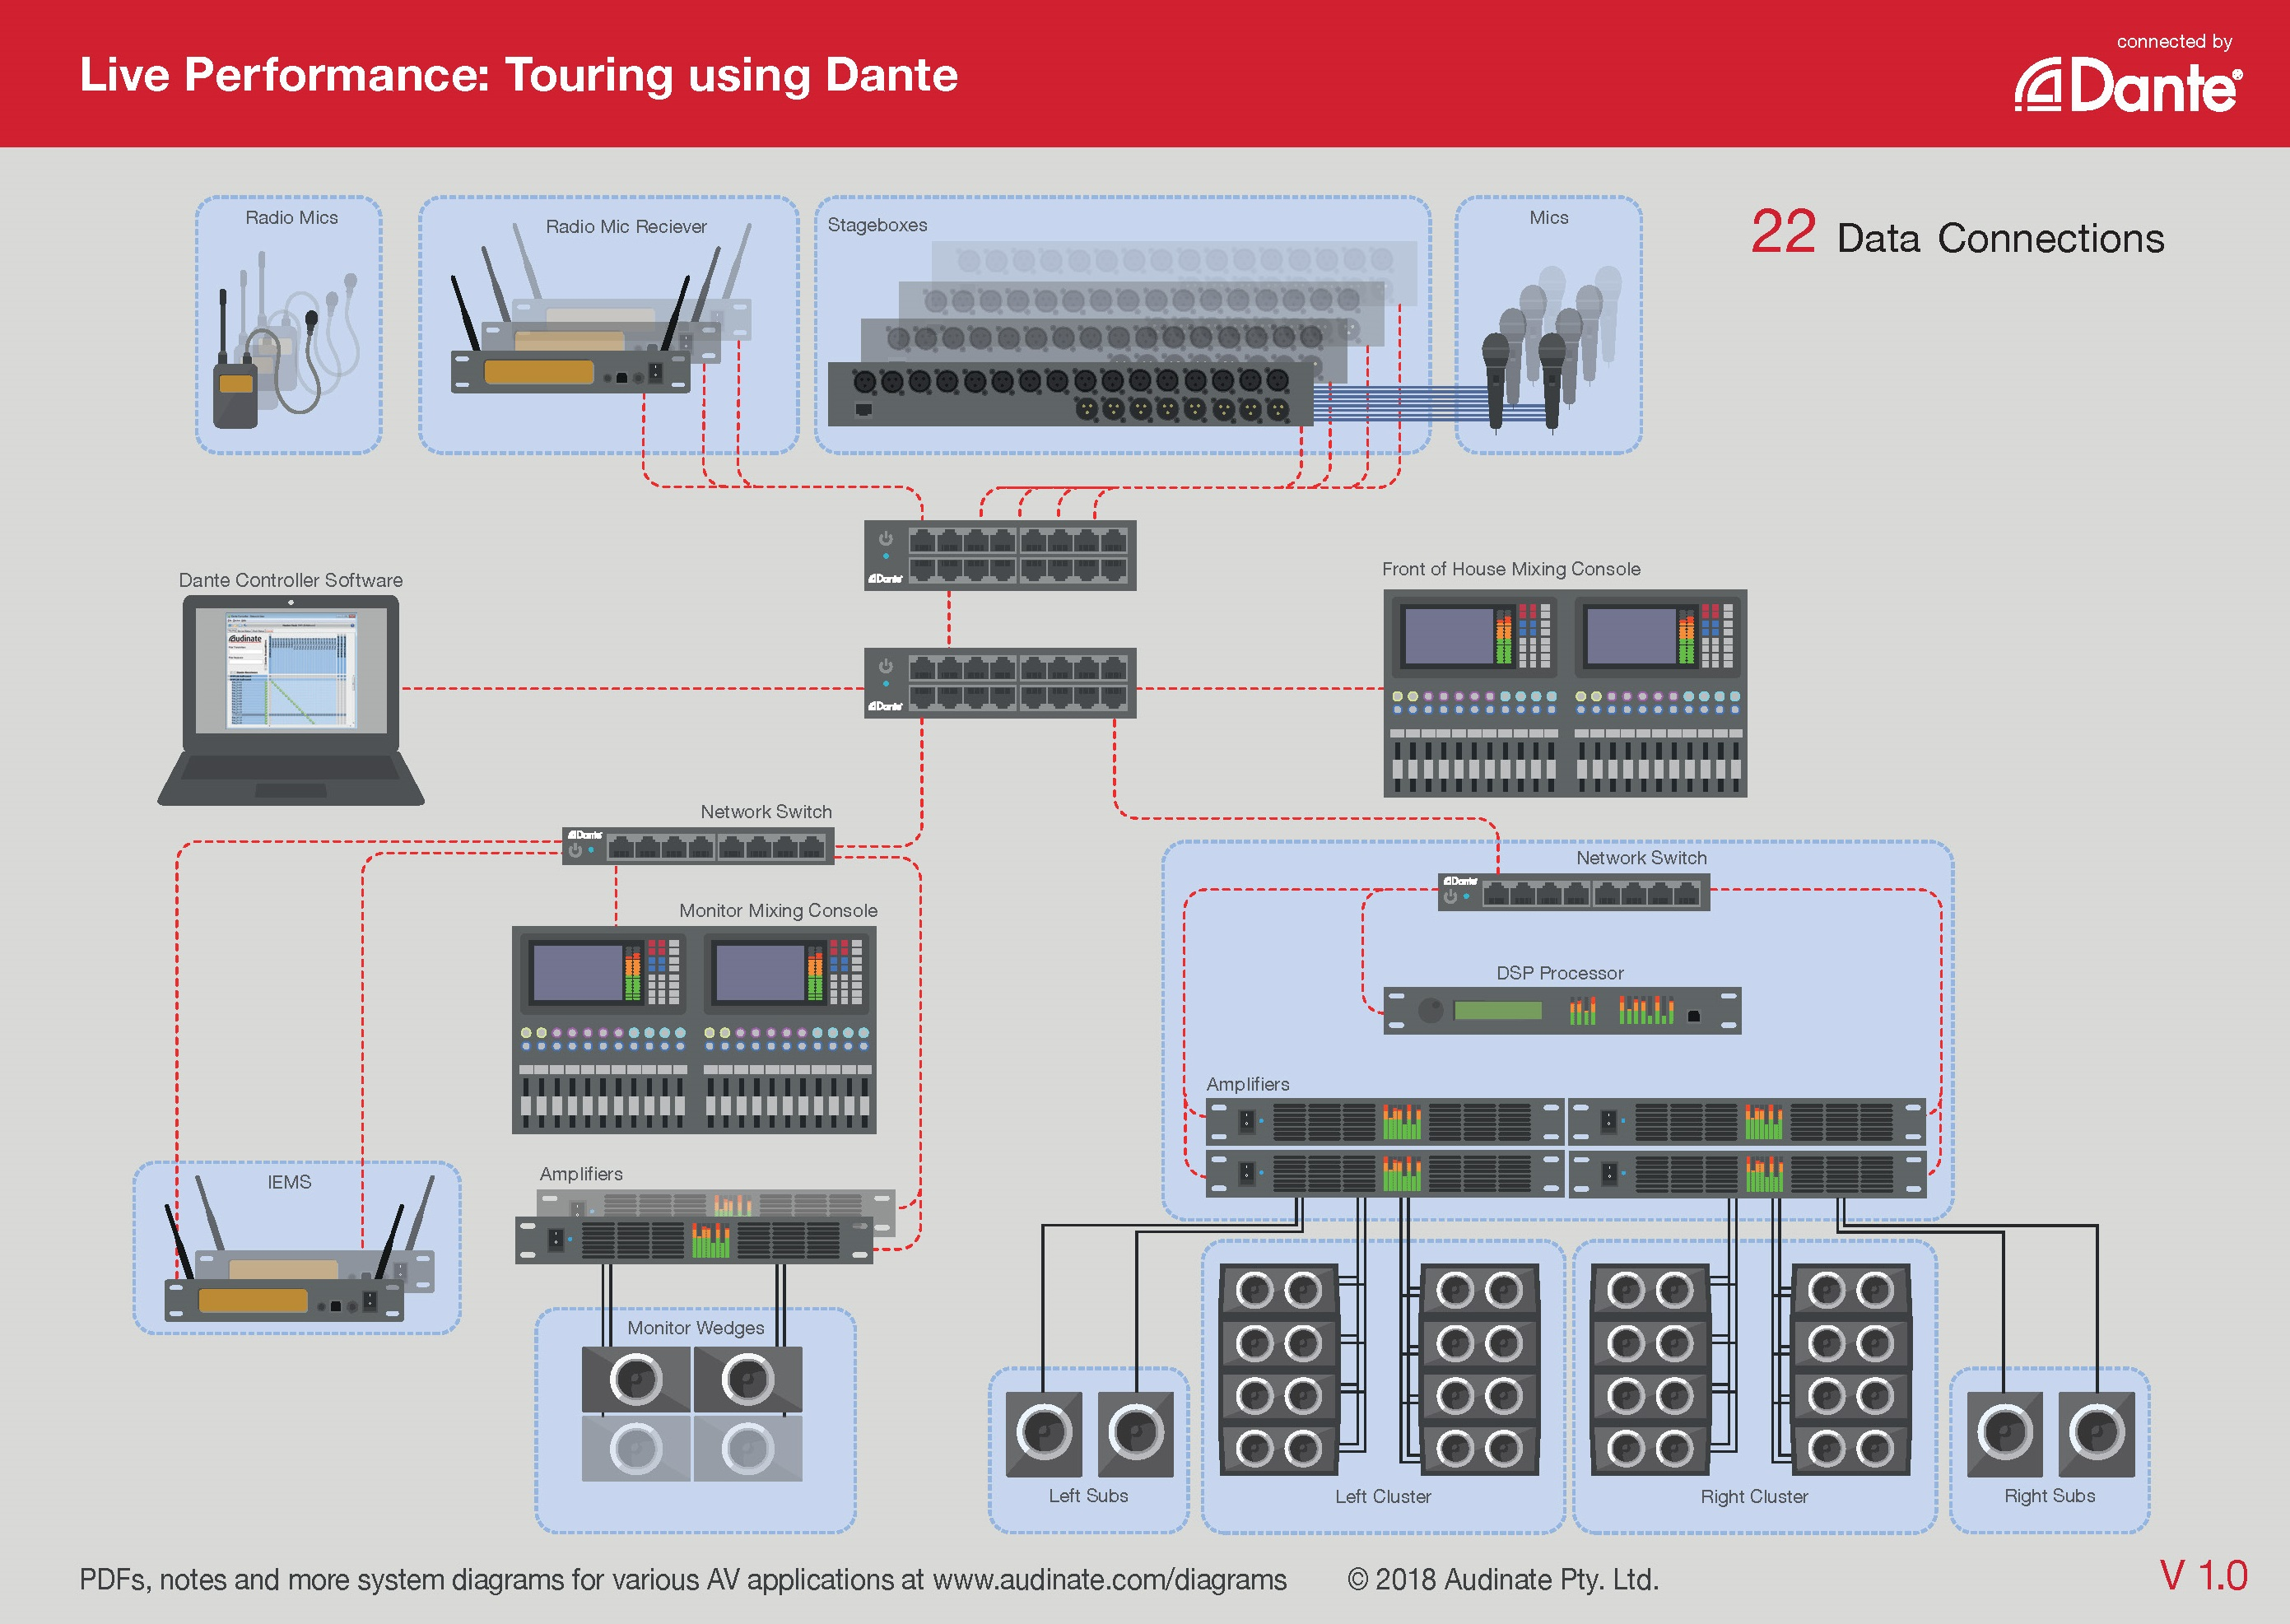
\includegraphics[width=\linewidth, keepaspectratio]{figures/live-dante.jpg}
	\caption{Példa Dante digitális kábelezésre \cite{APPLICATIONDIAGRAMSFORDANTESYSTEMS}}\label{fig:live-dante}
\end{figure}
%----------------------------------------------------------------------------

%----------------------------------------------------------------------------
\subsection{Martin Audio Wavefront Precision hangrendszer}
%----------------------------------------------------------------------------
\subsubsection{Martin Audio Display 2.3.4 b1 tervező szoftver \cite{DISPLAY23USERGUIDE}}
%----------------------------------------------------------------------------
Mielőtt bele fognánk a tervezési folyamatba, fontos megemlíteni, hogy a szoftver
eredetileg Intel alapú processzorokra lett tervezve és MatLab alapú. Ebből fakadóan
AMD Ryzen processzorokon habár elindult a szoftver, de nem volt stabil és a számítások során
minden esetben összeomlott, és használhatatlanul lassú volt. Személy szerint a saját gépem amivel dolgoztam
sajnos ilyen processzorral van szerelve ezért muszáj volt megoldást találni a problémára.
A Martin Audio hivatalos szoftveres támogatásához fordultam először, de sajnos nem tudtak segíteni.
Ezért a szoftver használatához
sok belefektetett óra olvasás után sikerült egy olyan MatLab CMD parancsot találnom, amivel
a szoftver elindul és használható.
Miután rájöttem a probléma gyökerére, ezt megosztottam velük, hogy a jövőben másoknak ne kelljen
ezzel a problémával szembesülniük.
A hiba az alábbi volt. Az új AMD Ryzen processzorok másfajta utasításkészletet használnak.
Ebből kifolyólag a MatLab 2015-s runtime alapú szoftver adta alaputasításokat nem tudta értelmezni a CPU.
A vezető szoftvermérnökkel való e-mail-es beszélgetésünk során megköszönte a probléma
megoldását, és nemsokkal a megoldásom megosztása után a hivatalos oldalra is felekerült
az indító parancsfájl. Az e-mailben további kollaborációra is adott lehetőséget.
A kompatibilitási problémát rögtön a script elején megoldottam,
mivel a következő parancs megadásával már használhatóvá válik a program: \texttt{set MKL\_DEBUG\_CPU\_TYPE=5} \newline
Ez a sor a program vezérlését AVX2-re állítja át, és mivel ezt az utasításkészletet már ismeri az AMD Ryzen processzor
is ezért a probléma már a múlté.
Az indító fájl további sorai optimalizálások a számítások gyorsítására, és a párhuzamosítására, ezzel jobban kihasználva
a rendelkezésre álló hardver erőforrásokat.
%----------------------------------------------------------------------------
\begin{lstlisting}[caption={A Display 2.3.4 b1 indító ".bat" scriptje AMD Ryzen processzorokhoz}, label=batcode, xleftmargin=\parindent]
    @echo off
    set PATH=%PATH%;C:\Program Files\Martin Audio\Display2_3_4_b1\application
    set MKL_DEBUG_CPU_TYPE=5
    set options=optimoptions('ga','UseParallel',true,'UseVectorized',false)
    set options=optimoptions('gamultiobj','UseParallel',true,'UseVectorized',false)
    set options=optimoptions('paretosearch','UseParallel',true)
    set options=optimoptions('particleswarm','UseParallel',true,'UseVectorized',false)
    set options=optimoptions('patternsearch','UseParallel',true,'UseCompletePoll',true,'UseVectorized',false)
    set options=optimoptions('surrogateopt','UseParallel',true)
    set GPUAcceleration=on
    start "Martin Audio" Display2_3_4_b1.exe
    pause
\end{lstlisting}
%----------------------------------------------------------------------------
\begin{figure}[H]
	\centering
	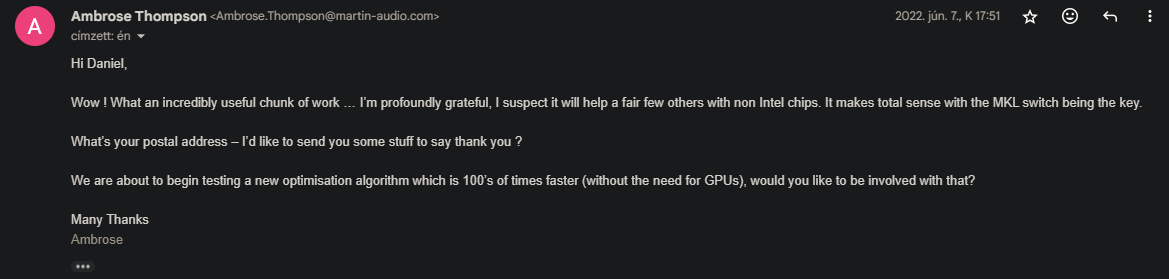
\includegraphics[width=\textwidth, keepaspectratio]{figures/ambrose_email.png}
	\caption{E-mail a Martin Audio vezető szoftvermérnökétől}
	\label{fig:ambrose_email}
\end{figure}
%----------------------------------------------------------------------------
Most, hogy már a szoftver használható és teljes mértékben működőképes, kezdjük el a tervezést.
A modellezés során a budapesti Millenáris B csarnoka lesz a referencia helyszín. Két LineArray rendszert fogunk
tervezni, mivel a terem hosszúsága és a lefedettség növelése miatt szükségünk lesz Delay kiegészítésre a fő hangrendszerhez.
Első lépésben a fő hangrendszert tervezem meg, ami oldalanként (bal és jobb) 8 darab WPC LineArray modulból fog állni.
Ez a láda 2 darab 10"-os mélysugárzót (LF), 2 darab 5"-os közép sugárzót (MF) és 4 darab 0.7"-os magassugárzót tartalmaz (HF).
Három utas Bi-amp meghajtású külső végfokot igénylő rendszer, ahol a mély tartományt (+1,-1) és a középmagas tartományt (+2,-2) külön kezeljük,
a négy pólusú Neutrik Speakon csatlakozókon keresztül.
A láda maximális hangnyomás szintje 135 dB, és 65 Hz-től 18 kHz-ig terjed a frekvencia átvitele +- 3 dB pontossággal. \cite{WPCUSERGUIDE}
%----------------------------------------------------------------------------
\begin{figure}[H]
	\centering
	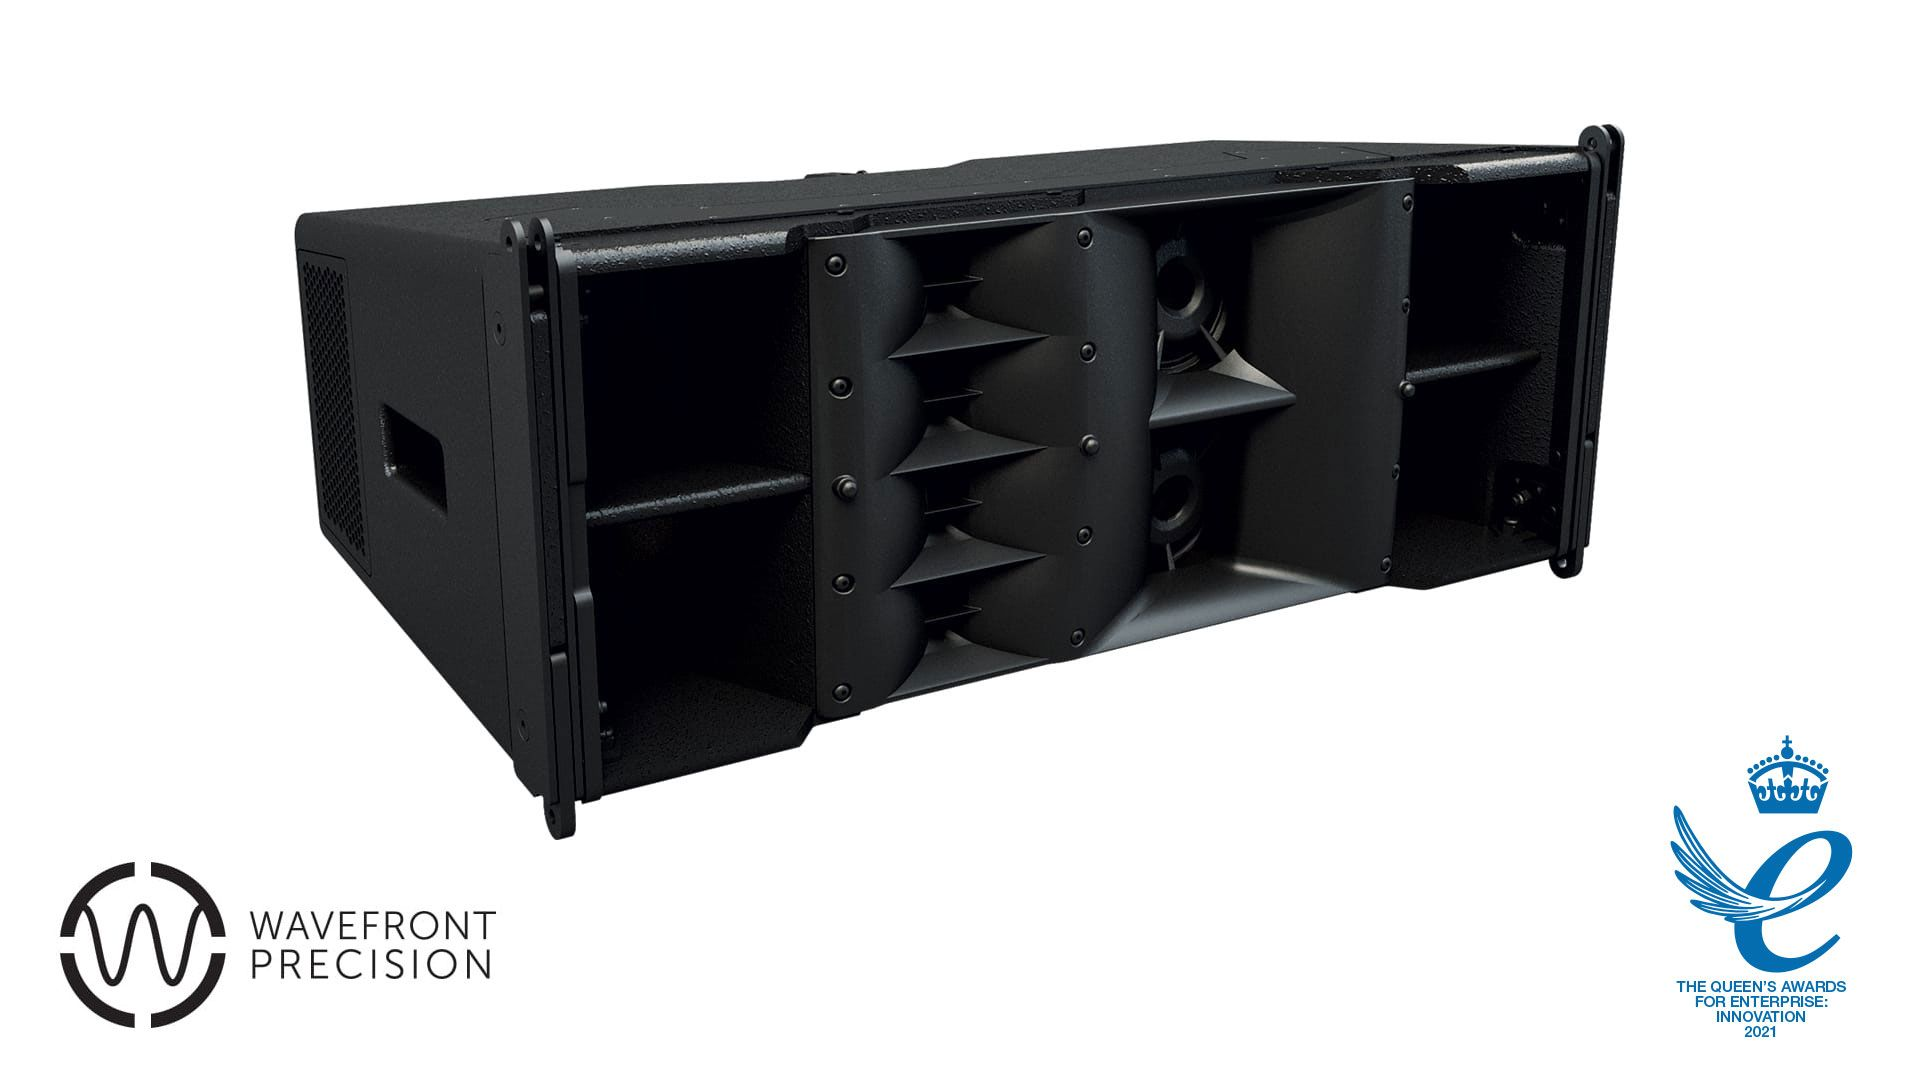
\includegraphics[width=80mm, keepaspectratio]{figures/wpc_front_view.jpg}
	\caption{Martin Audio WPC LineArray modul}\label{fig:wpc}
\end{figure}
%----------------------------------------------------------------------------
A program megnyitásakor a legelső lépés, hogy kiválasztjuk a termékpalettából a megfelelő hangrendszert.
Jelen esetben az előbbiekben említett WPC-t. A produkció igényei, a nagy létszámú közönség és a ládamennyiség miatt a rendszert
\textit{``riggelni''} fogjuk. (maximálisan 6 darab WPC-t lehet \textit{``stackelni''}, azaz a földre vagy mélyládákra helyezni)
A helyszín felmérése után a hangrendszer \textit{``riggelése''} lehetséges, mivel a csarnokban található tartószerkezet biztonságosan
és tartósan képes elviselni a rendszer súlyát.
A telepítés módja kiválasztása után megadjuk a szoftvernek a tervezni való hangláda mennyiséget, ez az esetünkben már említett 8 darab.
A hozzáadás gombra kattintva a elénk kerül a fő kezelőfelület, ahol a hangrendszert tudjuk lépésről lépésre tervezni.
%----------------------------------------------------------------------------
\begin{figure}[H]
	\centering
	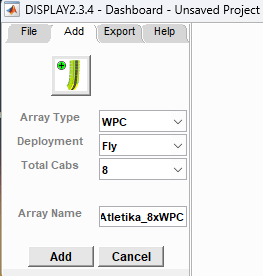
\includegraphics[width=40mm, keepaspectratio]{figures/display_wpc_0.png}
	\caption{Display 2.3.4 b1 kezdőképernyője (WPC)}\label{fig:display_wpc_0}
\end{figure}
%----------------------------------------------------------------------------
A tervezési folyamat öt részre osztható, amiket a szoftverben külön kezelünk.
Ezeket a \textit{``Slice''}, \textit{``Cover''}, \textit{``Splay''}, \textit{``Rig''} és \textit{``EQ''} kezelőfelületeken tudjuk elvégezni,
balról jobbra haladva. Mivel a különböző részegységek egymásra épülnek, ezért fontos a sorrend betartása.
(tervezés utáni módosításokra természetesen van lehetőség, de az adott projekt első tervezési folyamata során ezeket a lépéseket kell követni)
%----------------------------------------------------------------------------
\begin{figure}[H]
	\centering
	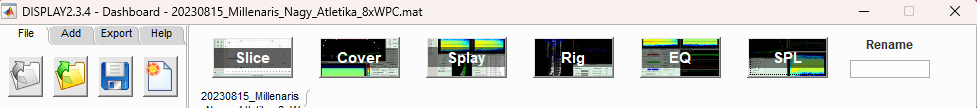
\includegraphics[width=\textwidth, keepaspectratio]{figures/display_wpc_0_1.png}
	\caption{Display 2.3.4 b1 fő kezelőfelülete (WPC)}\label{fig:display_wpc_0_1}
\end{figure}
%----------------------------------------------------------------------------
A \textit{``Slice''} panelen meghatározzuk a rendszer fizikai pozícióját térben. A csarnok
pontos lemodellezése érdekében a mérésekhez lézeres távolságmérőt használtam.
Mivel minden egyes rendezvényen más és más a különböző elemek elhelyezkedése, ezért a
rendszert minden alkalommal újra kell tervezni, még akkor is ha maga a helyszín nem változik.
\textit{``Vertex''} pontok segítségével tudjuk a méreteket és a pozíciókat meghatározni.
A 2D-s modellen figyelembe kell venni a terem önálló méretén kívül a színpadod és a színpad mögötti területet is.
A rajznak tartalmazni kell azokat a falfelületeket is amelyeknél a hangvisszaverődést minimalizálni szeretnénk,
ennek az optimalizáció későbbi fázisában lesz jelentősége.
A terem pontos rajza után még két fontos paramétert kell megadni ezen a felületen.
El kell helyeznünk magát a hangrendszert a teremben, és meg kell határoznunk milyen magasra szeretnénk a rendszert emelni.
Mivel a csarnok rendkívül hosszú, és a adottságai megengedik, ezért a rendszert minél magasabbra szeretnénk emelni,
a jobb lefedettség érdekében.
A másik fontos paraméter az optimalizációhoz, a közönség területének meghatározása. Kezdő és végpont segítségével
tudjuk a területet meghatározni, ahol a hallgatóközönség tartózkodni fog.
%----------------------------------------------------------------------------
\begin{figure}[H]
	\centering
	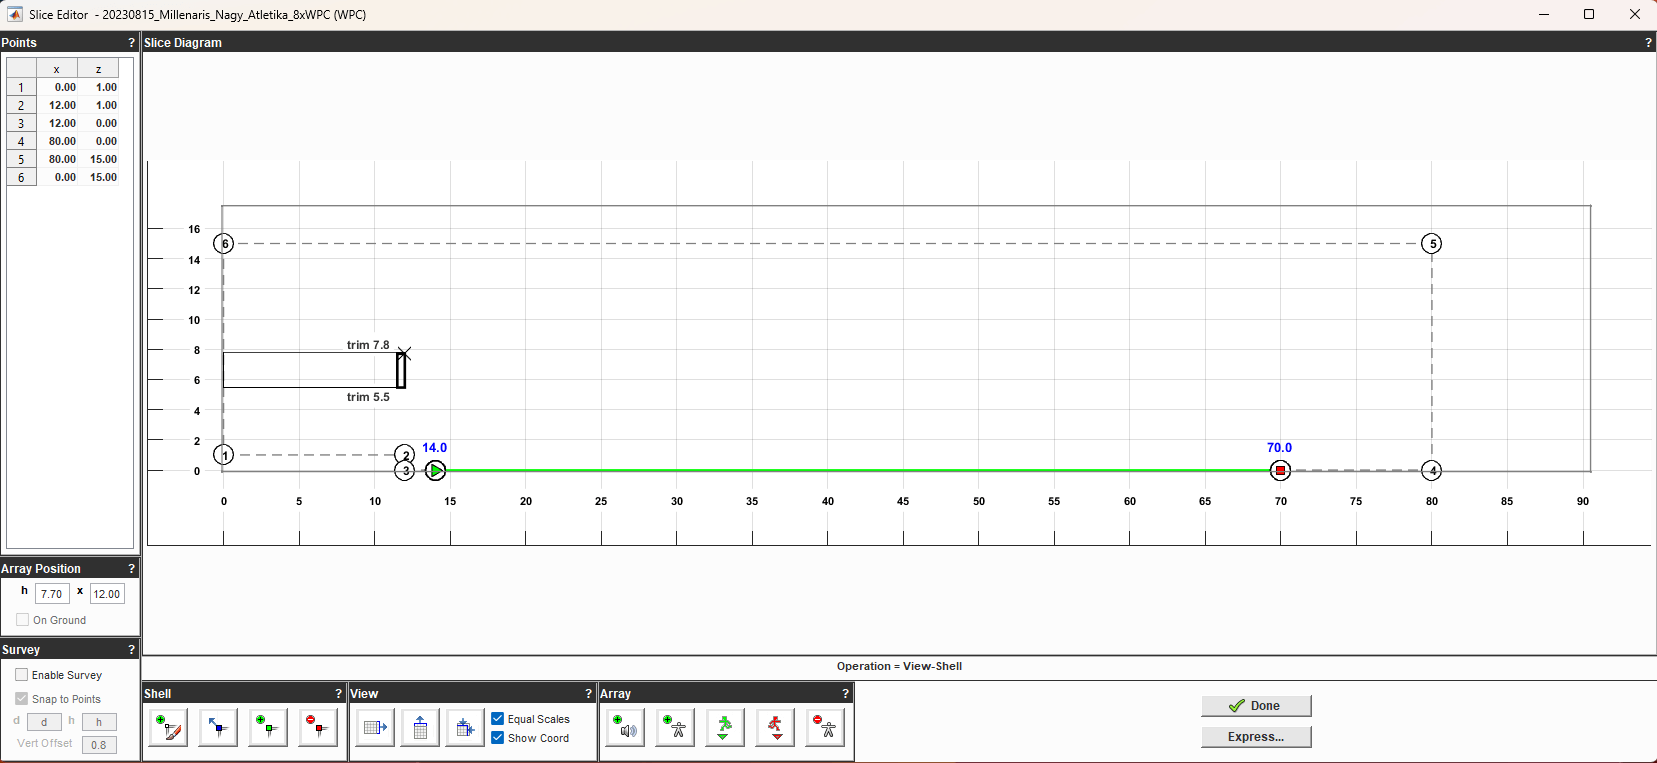
\includegraphics[width=\textwidth, keepaspectratio]{figures/display_wpc_1.png}
	\caption{Display 2.3.4 b1 \textit{``Slice''} kezelőfelülete (WPC)}\label{fig:display_wpc_1}
\end{figure}
%----------------------------------------------------------------------------
A következő lépések a \textit{``Cover''} kezelőfelületen történnek.
Első és legfontosabb beállítás amit el kell végezni, hogy a hallgatóság az esemény során ülni vagy állni fog-e.
Lehetőségünk van a nézőteret különböző részekre is osztani, amennyiben a rendezvény során különböző helyeken
eltérő típusú részeket szeretnénk egyenletesen lefedni. Lehetőség van egyedi magasság beállítására is,
de jelen esetben a közönség egyhangúan állva fogja hallgatni a produkciót, ezért a \textit{``Standing''} opciót választottam.
Az előző lépésben elkészített rajzunkon definiálhatunk a program számára három fő régiót.
\newline Ezek az alábbiak:
%----------------------------------------------------------------------------
\begin{itemize}
	\item \textit{``Non Audience''} - a közönség területén kívül eső terület
	\item \textit{``Audience''} - a közönség területe
	\item \textit{``Hard Avoid''} - a közönség területén kívül eső terület, ahol a hangvisszaverődést szeretnénk minimalizálni
\end{itemize}
%----------------------------------------------------------------------------
Jelen esetben a fő hangrendszernél nem jelöltem meg a \textit{``Hard Avoid''} területet, mivel a teremben az első olyan felület
ami a hangvisszaverődést okozna már olyan távol helyezkedik el a hangrendszertől, hogy a hangvisszaverődés már nem okoz problémát.
A következő lépéseket előkészítve meg kell határoznunk a hangrendszertől egy adott távolságra lévő pontot a teremben,
amit referencia pontként fogunk használni. Ezt a pontot a \textit{``Move Ref''} gombra kattintva tudjuk megadni,
vagy manuálisan beírva az X és Y koordinátákat. Automatikusan a terem közepére van pozícionálva a referencia pont, de
ezt erősen ajánlott mozgatni attól függően mit szeretnénk elérni. Jelen esetben a mix pultot fogjuk a referencia pontnak megadni.
A \textit{``Start''} és \textit{``Stop''} mezőkben meg kell adnunk, hogy a referencia ponttól véve mekkora hangnyomás
deltával szeretnénk dolgozni. Ez azt jelenti, hogy a kezdő, a referencia és a végpont közötti hangnyomás hány dB-el térhet el egymástól.
Ezt az értéket a szoftver az eddig megadott információk alapján automatikusan kiszámolja, de manuálisan is megadhatjuk.
Az automatikus számítás az esetek többségében megfelelő eredményt ad, ezért most is ezt választottam.
A \textit{``Target SPL''} mezőben megadhatjuk a referencia ponton elérni kívánt hangnyomás szintet.
Így a rendszer \textit{``Gain''} struktúrája úgy lesz beállítva, hogy a referencia ponton 0 dBu bemeneti szint mellett elérjük a megadott hangnyomás szintet.
Magas frekvenciák csökkennek ahogy a távolság nő a forrástól, azaz a hangrendszertől.
Ha egyenletes frekvencia választást szeretnénk elérni nagyobb távolságokon, akkor a rendszernek nagyobb energiára lenne szüksége
a magas frekvenciákon, és kifutna a dinamika tartalékból, ezért jobb megoldás, ha a magas frekvenciák fokozatosan csökkennek a távolság növekedésével.
Beállíthatjuk a levegő veszteség kompenzációját, teljesen balra állítva nincs kompenzáció (figyelmen kívül hagyva a levegő abszorpcióját).
Teljesen jobbra állítva a maximális kompenzáció (a rendszernek 17dB headroom-ra van szüksége, hogy egyenes választ kapjunk).
Viszont ezekből az következik, hogyha túlságosan sok a kompenzáció, akkor a rendszernek nem lesz elég dinamika tartaléka, és a hang torzulni fog.
A változások hatását a \textit{``Target Response''} ábrán láthatjuk.
Ahhoz, hogy a számítások pontosak legyenek, elengedhetetlen, hogy pontosan megadjuk a környezeti változókat,
a hőmérsékletet, a páratartalmat és a légnyomást. Ezeket a paramétereket a \textit{``Edit''} gombra kattintva tudjuk megadni.
Jelen esetben mivel a teremben alapból is meleg van, a mérés időpontjában 28 fok, és a rendezvény során a közönség is melegíti a termet,
ezért a hőmérsékletet harminc fokra állítottam.
A páratartalom értéke a méréskor 57\%-os volt, de én 65\%-ra állítottam, mivel a rendezvény során a közönség által kibocsátott
vízgőz miatt a páratartalom nagy valószínűséggel magasabb lesz ennél. A légnyomás értékét pedig a helyi időjárás jelentésből vettem, ami
azon a napon 101800 Pa volt. Ezek beállítása után mivel az adott hangládához a gyári beállítások nagyon jók, ezért nem változtattam rajtuk,
a 14-es érték egyenletes és dinamikus hangvisszaadást biztosít.
%----------------------------------------------------------------------------
\begin{figure}[H]
	\centering
	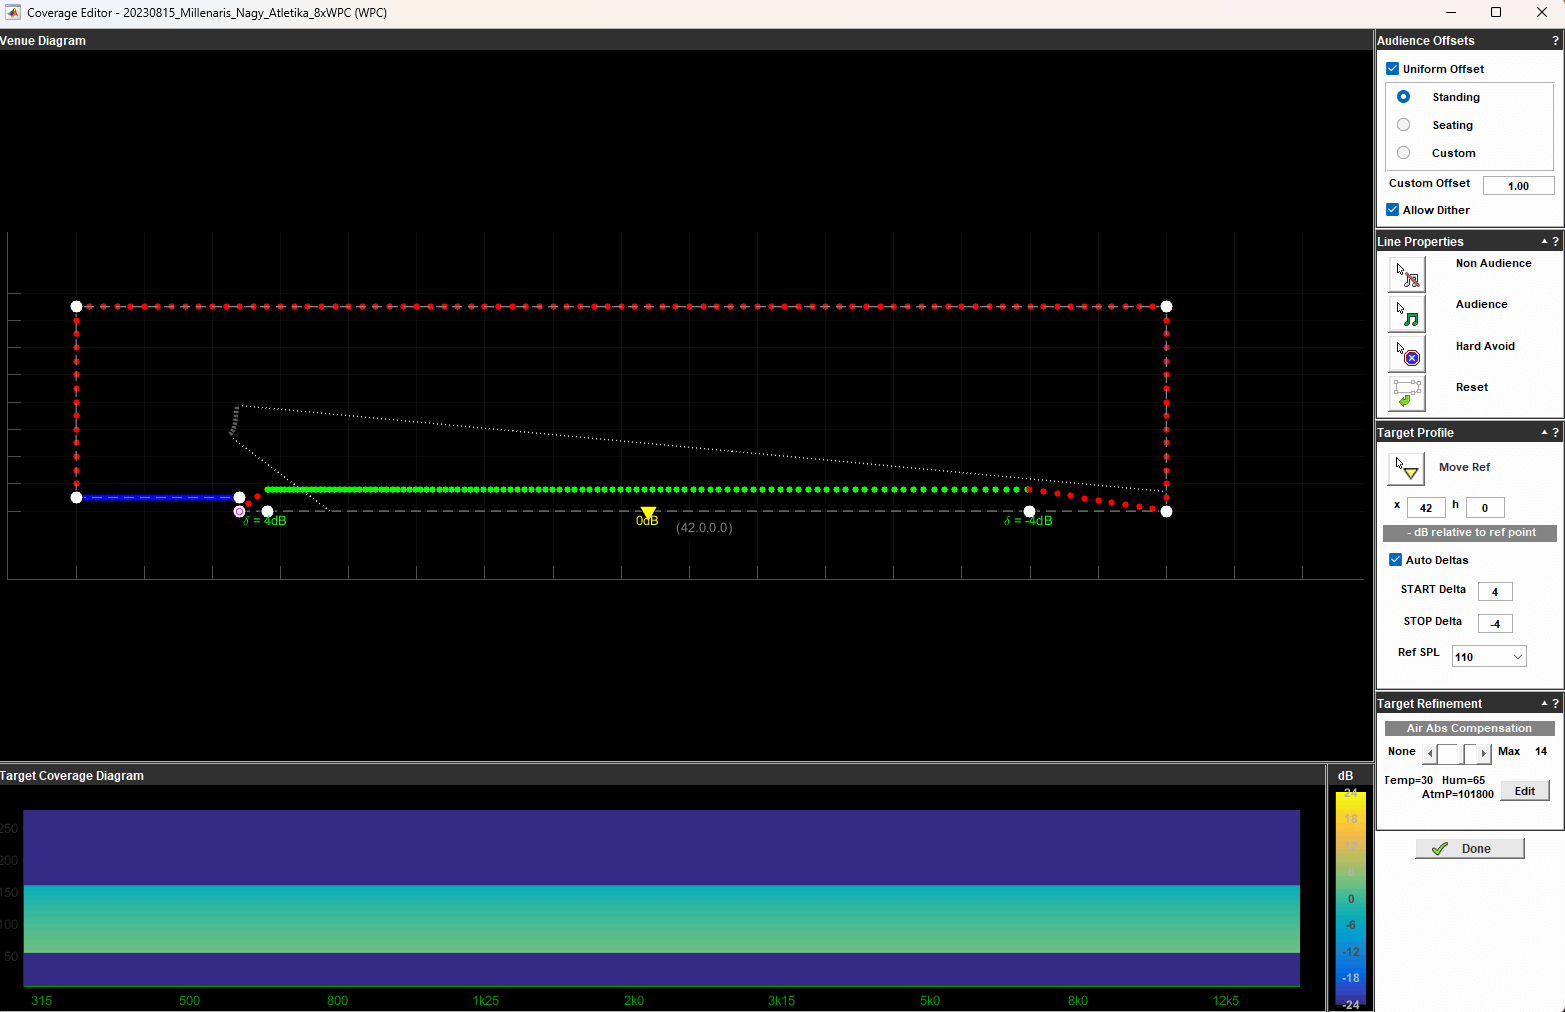
\includegraphics[width=\textwidth, keepaspectratio]{figures/display_wpc_2.png}
	\caption{Display 2.3.4 b1 \textit{``Cover''} kezelőfelülete (WPC)}\label{fig:display_wpc_2}
\end{figure}
%----------------------------------------------------------------------------
Miután a \textit{``Cover''} kezelőfelületen elvégeztük a szükséges beállításokat, a \textit{``Splay''} kezelőfelületen folytatjuk a tervezést.
Az optimalizáció ezen részén a hangrendszert fogjuk a hallgatóság területére irányítani, a fokolási szögek beállításával.
A szoftver által biztosított optimalizációs algoritmus a lehető legjobb lefedettségre törekszik a tervezett területen.
Lehetőség van az optimalizáció súlyozási tényezőinek beállítására, de jelen esetben a gyári beállításokat használtam.
Amennyiben módosítani szeretnénk a súlyozást a \textit{``Target'} és a \textit{``Leakage''} mezőkben tudjuk megadni a súlyozási tényezőket.
A \textit{``Target''} mezőben megadott érték a közönség terület súlyozása,
a \textit{``Leakage''} mezőben megadott érték pedig a közönség területén kívül eső szivárgás súlyozása.
Az \textit{``Alow Polish''} opció engedélyezi a szoftvernek, hogy egy második körben finom hangolja a splay szögeket az első próbálkozás után.
Ezt az opciót előnyös bekapcsolni, mivel a szoftver így pontosabb eredményt tud produkálni, ezért ezt a beállítást mindig használom.
A \textit{``Max Time''} mezőben megadhatjuk, hogy a szoftvernek mennyi idő álljon rendelkezésére az optimalizáció elvégzéséhez.
Mivel a mai modern számítógépek olyan gyorsak, hogy a szoftver általában 1-2 perc alatt elvégzi az optimalizációt, ezért ezt az értéket
nem szoktam módosítani. A \textit{``Max Time''} mezőben megadott érték másodpercben értendő.
%----------------------------------------------------------------------------
\begin{figure}[H]
	\centering
	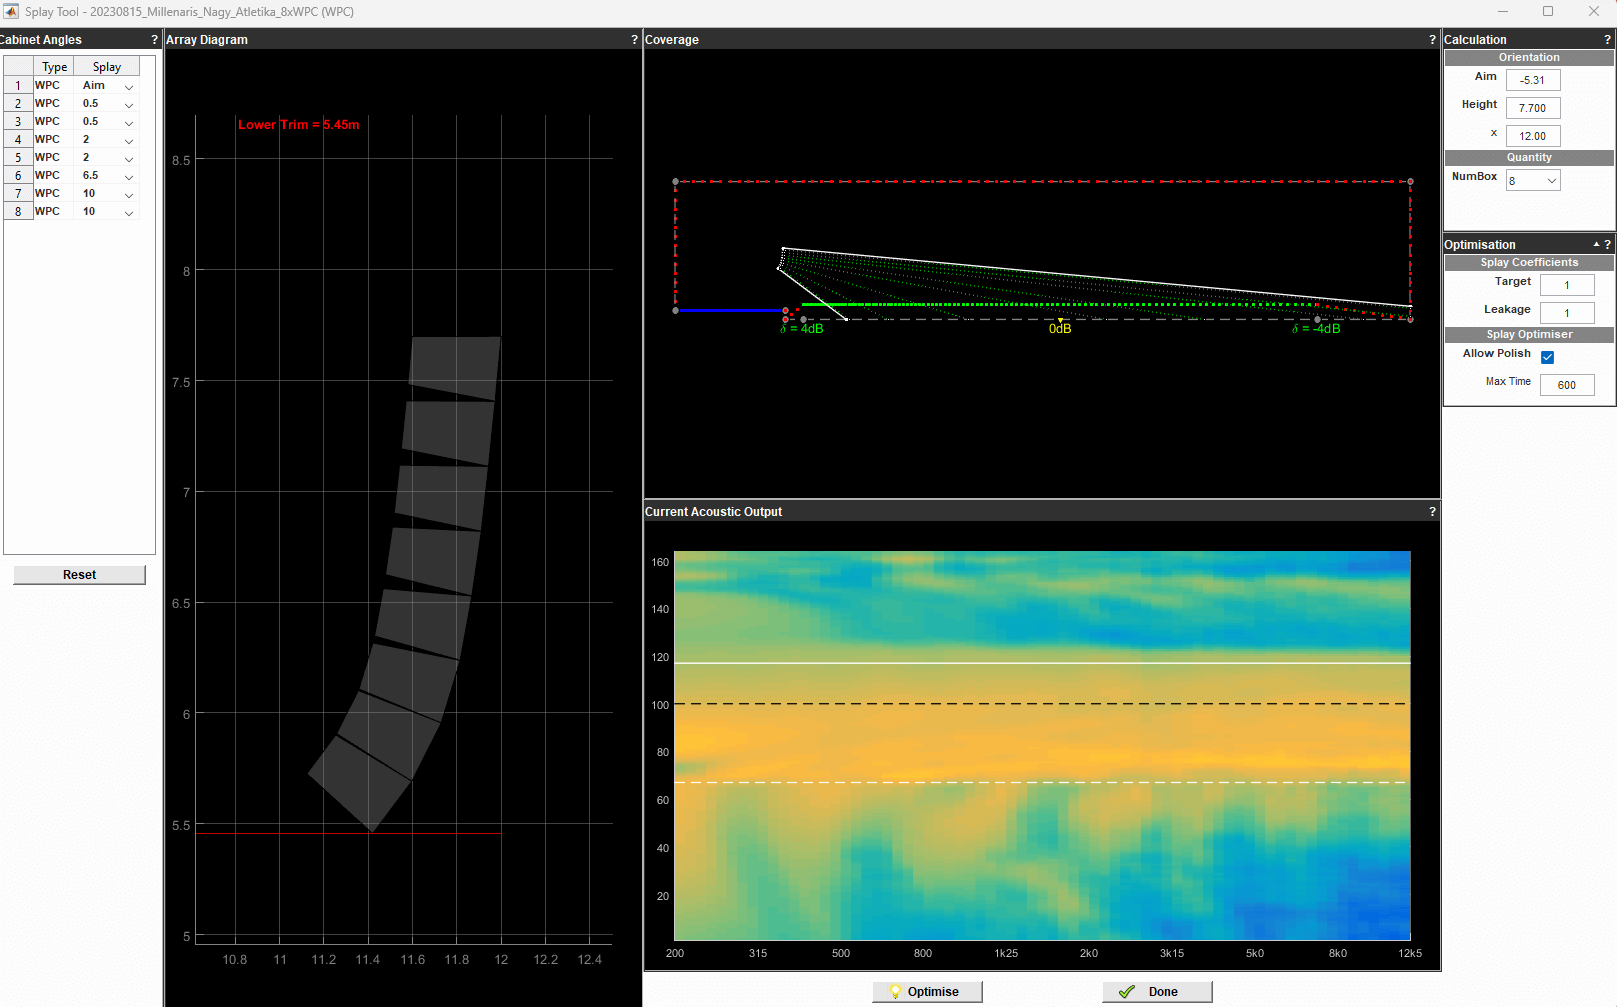
\includegraphics[width=\textwidth, keepaspectratio]{figures/display_wpc_3.png}
	\caption{Display 2.3.4 b1 \textit{``Splay''} kezelőfelülete (WPC)}\label{fig:display_wpc_3}
\end{figure}
%----------------------------------------------------------------------------
A következő lépés a \textit{``Rig''} kezelőfelületen történik. Ez a felület elsősorban az eddig elkészített
rendszerünket fogja megjeleníteni térben. Elsődleges beállítási paraméter ezen a panelen, hogy egy vagy két pontos
rögzítést szeretnénk-e használni. Jelen esetben egy pontos  rögzítést fogunk használni. Amennyiben valamilyen okból
szeretnénk változtatni a rendszer fizikai elhelyezkedésén, még megtehetjük, de ez a lépés ezen a ponton már nem ajánlott.
Bármely kis apró változtatás kardinálisan más végeredményhez vezethet. A tervezési folyamatot újra kell kezdeni, ellenkező esetben
a szoftver nem fogja tudni a megfelelő eredményt produkálni, és a rendszerünk nem úgy fog viselkedni a valóságban, ahogy azt mi szeretnénk.
A hangrendszer függesztéséhez és összeszereléséhez az összes információ megtalálható itt. Gondolva itt a riggvas fokolási helyére,
a ládák közti szögekre, a rendszer legfelső és legalsó pontjára.
Ezeken az információkon kívül még a rendszer súlyát és súlypontját is megkapjuk.
Esetünkben a teljes súly 289 kilogramm, amit a csarnok tartószerkezete biztonságosan elbír, valamint az egy tonnás emelőkapacitású
láncos emelők is képesek biztonságosan emelni. A súlypont a rendszer relatíve közepén helyezkedik el, ami stabil függesztést tesz lehetővé.
Ezek után a rendszert az említett paraméterek alapján össze építjük, figyelve az összes program által megadott információra.
%----------------------------------------------------------------------------
\begin{figure}[H]
	\centering
	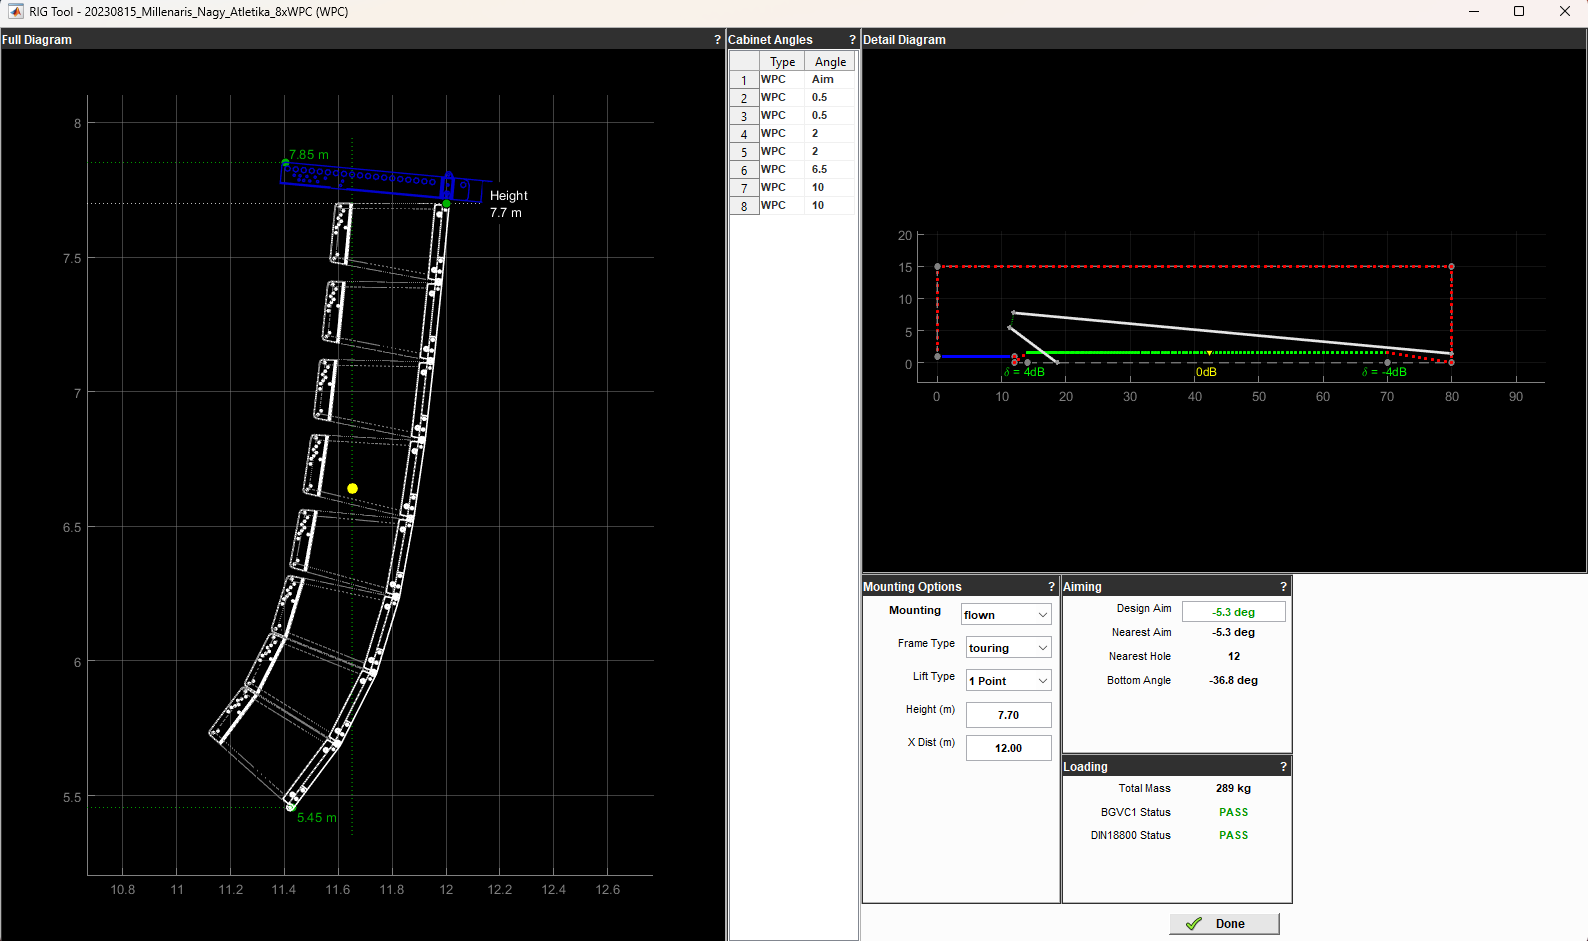
\includegraphics[width=\textwidth, keepaspectratio]{figures/display_wpc_4.png}
	\caption{Display 2.3.4 b1 \textit{``Rig''} kezelőfelülete (WPC)}\label{fig:display_wpc_4}
\end{figure}
%----------------------------------------------------------------------------
Az utolsó lépés mielőtt ki tudnánk menteni a tervezett rendszert, az a \textit{``EQ''} kezelőfelületen történik.
Ha a \textit{``Cover''} kezelőfelületen már megadtuk a környezeti változókat, akkor ezt már nem kell újra megtennünk,
mivel a szoftver automatikusan átveszi az ott megadott értékeket. Beállíthatjuk az alsó és felső határfrekvenciákat, de mivel
a program a kiválasztott hangrendszerhez tartozó gyári beállításokat automatikusan betölti, ezért ezeket az értékeket sem kell módosítani.
Amit viszont érdemes és erősen ajánlott módosítani, az a \textit{``Freq Res''} és a \textit{``Space Res''} értékek. Az előbbi a
frekvencia felbontást, az utóbbi pedig a térbeli felbontást jelenti. Ezek az értékek határozzák meg, hogy a szoftver milyen 
felbontásban végezze el a számításokat. Minél kisebb értéket adunk meg, annál pontosabb eredményt fogunk kapni, viszont a számítások
hosszabb ideig fognak tartani. A \textit{``Freq Res''} értékét 1-re, a \textit{``Space Res''} értékét pedig szintén 1-re állítottam, mivel
ez az elérhető legnagyobb felbontás, és a számításokat is a lehető legpontosabban szeretném elvégezni. A gyári érték mindegyiknél a kettő.
Minél pontosabbak a számítások, annál jobban fog viselkedni a rendszer a valóságban és egyenletesebb hangvisszaadást fog produkálni.
Ha már a kiegyensúlyozott hangvisszaadásnál tartunk, akkor a \textit{``Resolution''} panelen meg kell adnunk, hogy milyen
konfigurációban szeretnénk használni a rendszert. A WPC szériás hangládákat tudjuk akár egyesével hajtani, azaz egy láda egy végfok csatorna
párral (mivel Bi-Amp hangládáról beszélünk). De a gyártó lehetőséget biztosít arra is, hogy a ládákat párosával vagy hármasával is hajtsuk.
Ennek költséghatékonysági és rugalmassági előnyei vannak, viszont a hangvisszaadás kevésbé lesz egyenletes. Jelen esetben 
az arany középutat választottam, és párosával fogom hajtani a ládákat. Így a WPC rendszer összesen 4 darab iK42 végfokot fog igényelni, ami 
16 darab végfokcsatornát jelent. A WPC rendszer csak iK42 végfokkal hajtható, a 8 csatornás iK81 végfokkal nem kompatibilis.
Lehetőség van az optimalizációs algoritmus befolyásolására is, a három előbbiekben már definiált súlyozási tényezők segítségével.
A fő hangsúlyt a \textit{``Target''} súlyozásra helyeztem, mivel a közönség területén szeretném a lehető legjobb hangvisszaadást elérni,
ezért 60\%-os súlyozást adtam neki.
A \textit{``Hard Avoid''} és a \textit{``Leakage''} súlyozását 20\%-ra állítottam.
Továbbá mindhárom résznek megadhatjuk mekkora hangnyomás értéket szeretnénk elérni a tervezett területen. Ezeket az értékeket
nem szükséges módosítani, mivel a gyári értékek megfelelőek, de ha mégis szeretnénk, akkor megtehetjük.
A paraméterezés után az optimalizáció után megkapjuk a teljes rendszer EQ beállítását és vizuális ábrázolást kapunk 
a referencia értéktől való eltérésekről.
%----------------------------------------------------------------------------
\begin{figure}[H]
	\centering
	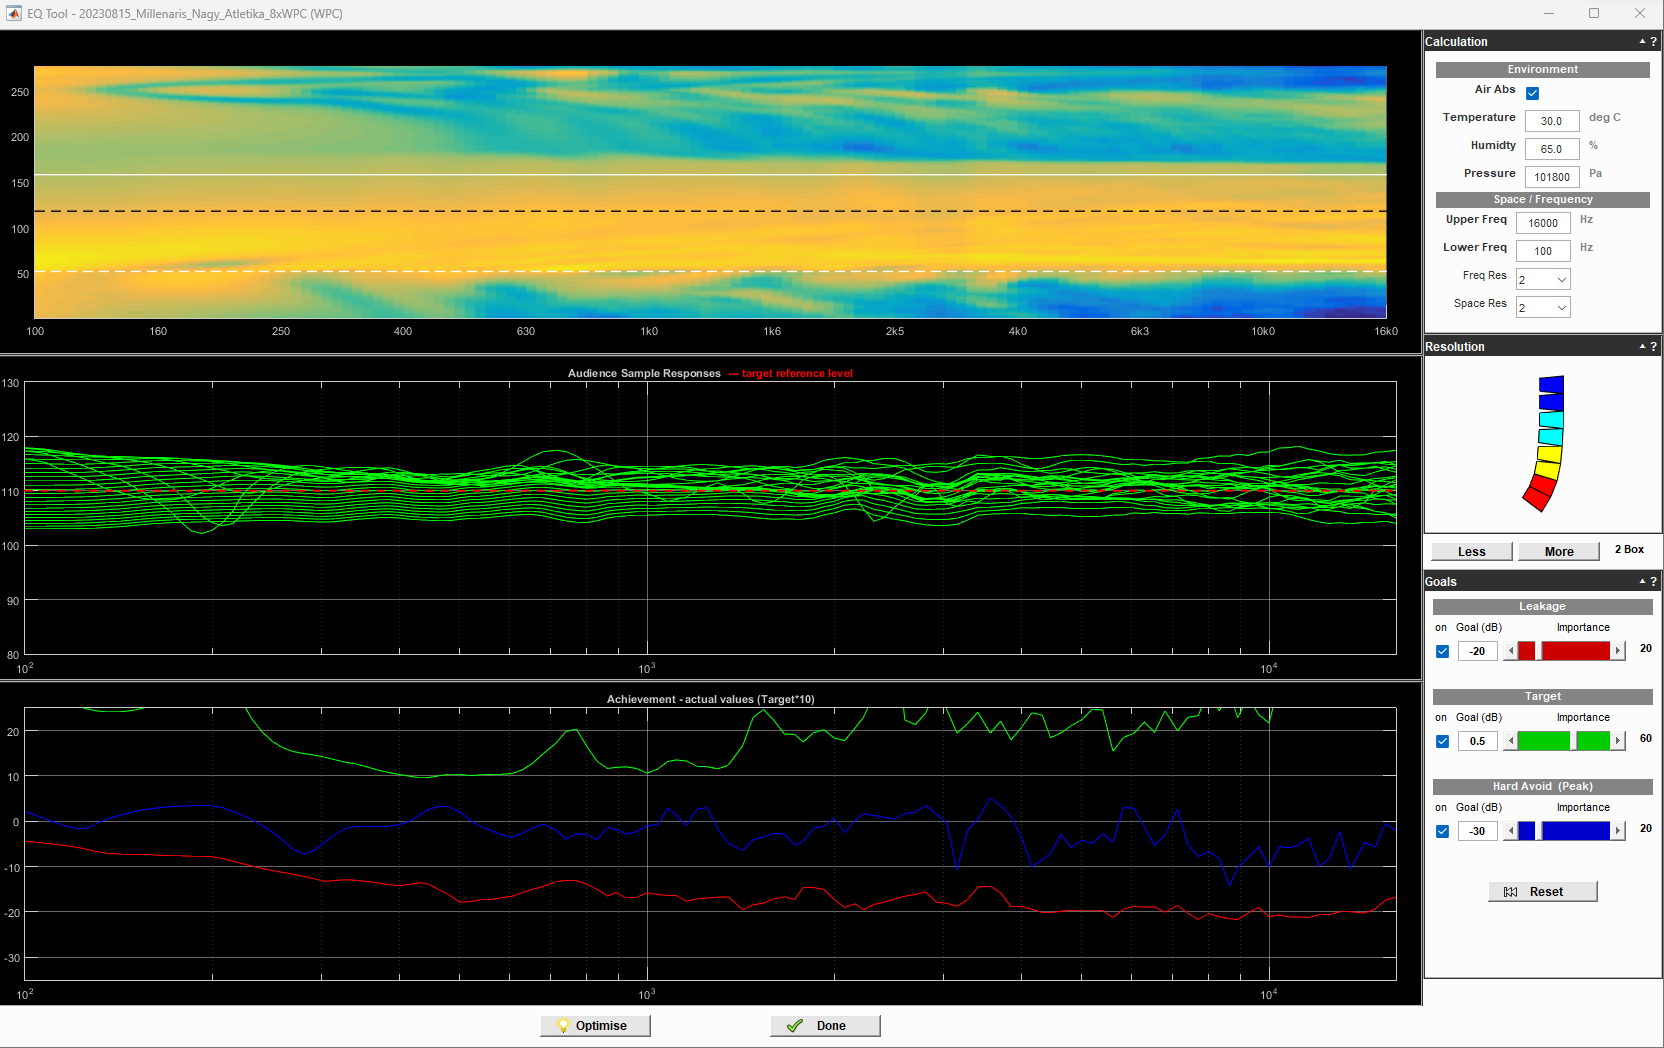
\includegraphics[width=\textwidth, keepaspectratio]{figures/display_wpc_5.png}
	\caption{Display 2.3.4 b1 \textit{``EQ''} kezelőfelülete (WPC)}\label{fig:display_wpc_5}
\end{figure}
%----------------------------------------------------------------------------
%Amennyiben szeretnénk megtekinteni a tervezett rendszer teljesítményét amit a program számított ki, 
%akkor az \textit{``SPL''} kezelőfelületen, az \textit{``Index Plot''}-on a bal egeret nyomva tartva
%tudunk virtuálisan mozogni a teremben, és megtekinthetjük a számított hangnyomás és frekvencia eloszlás értékeket.
%Ha mindent rendben találunk és nincsenek kivetnivalóink a tervezett rendszerrel kapcsolatban, akkor
%sikeresen megterveztük a hangrendszert, és elmenthetjük a projektet.
%A mentés során egy MAT kiterjesztésű fájlt fogunk kapni, segítségével később bármikor újra megnyithatjuk a projektet,
%ha ugyan azon a helyszínen dolgozunk, gyorsabban és egyszerűbben tudjuk a rendszert újra tervezni, a szükséges
%módosításokat elvégezni.
%----------------------------------------------------------------------------
%\begin{figure}[H]
%	\centering
%	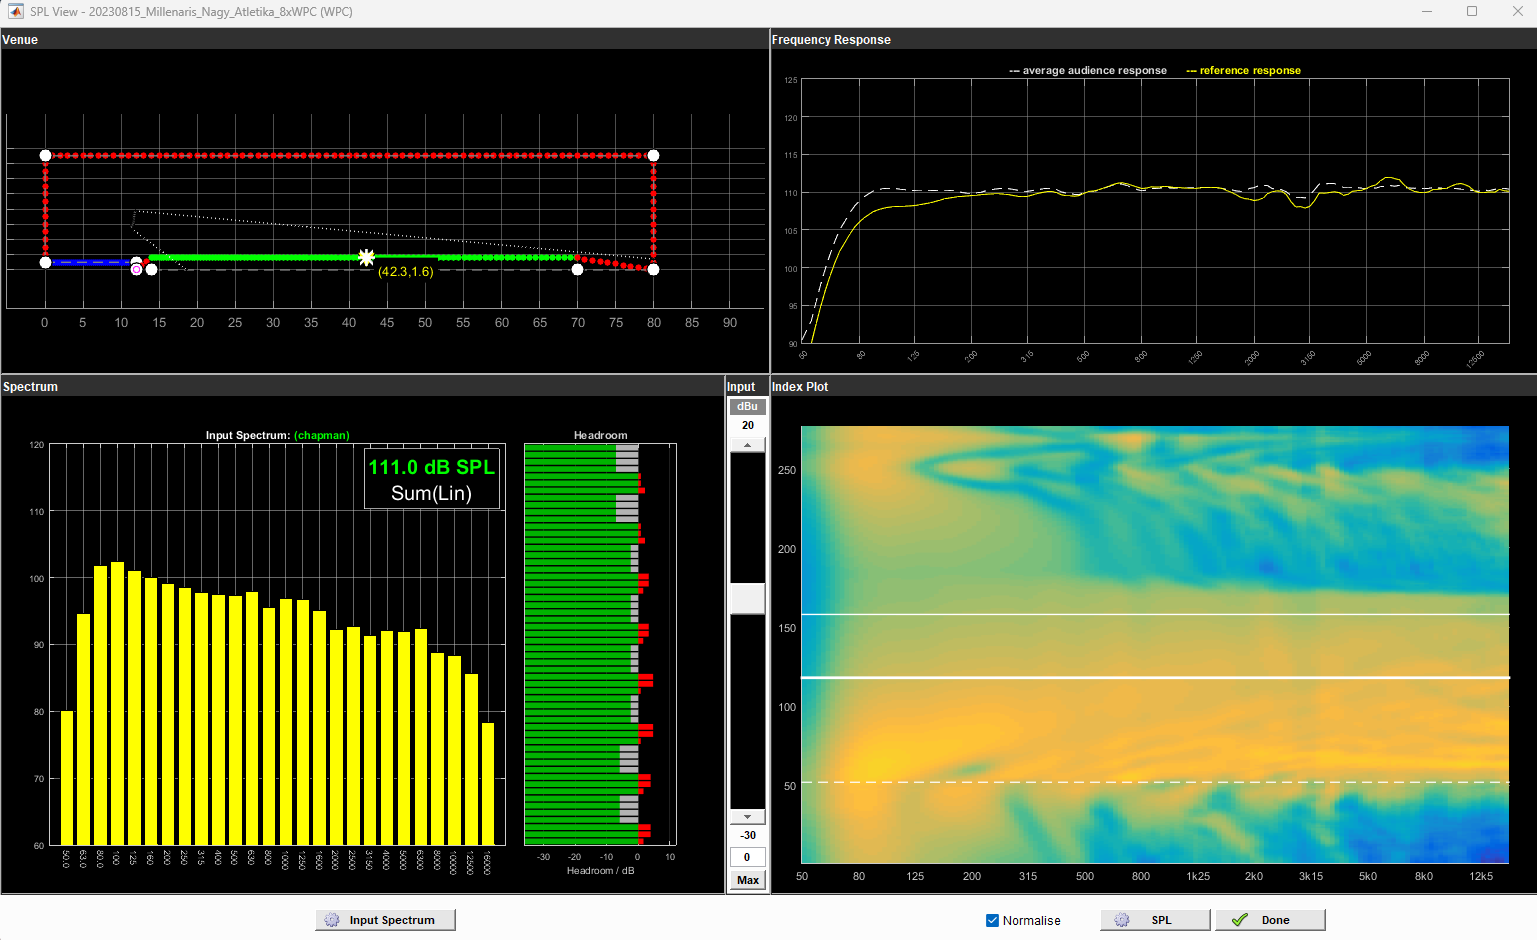
\includegraphics[width=\textwidth, keepaspectratio]{figures/display_wpc_6.png}
%	\caption{Display 2.3.4 b1 \textit{``SPL''}kezelőfelülete (WPC)}\label{fig:display_wpc_6}
%\end{figure}
%----------------------------------------------------------------------------
Az utolsó dolgunk ebben a programban mielőtt tovább lépünk, hogy exportáljuk a tervezett rendszert.
Az exportálás során egy D2P kiterjesztésű fájlt fogunk kapni, amit a VU-NET szoftver fog tud majd importálni a későbbiekben.
%----------------------------------------------------------------------------
\begin{figure}[H]
	\centering
	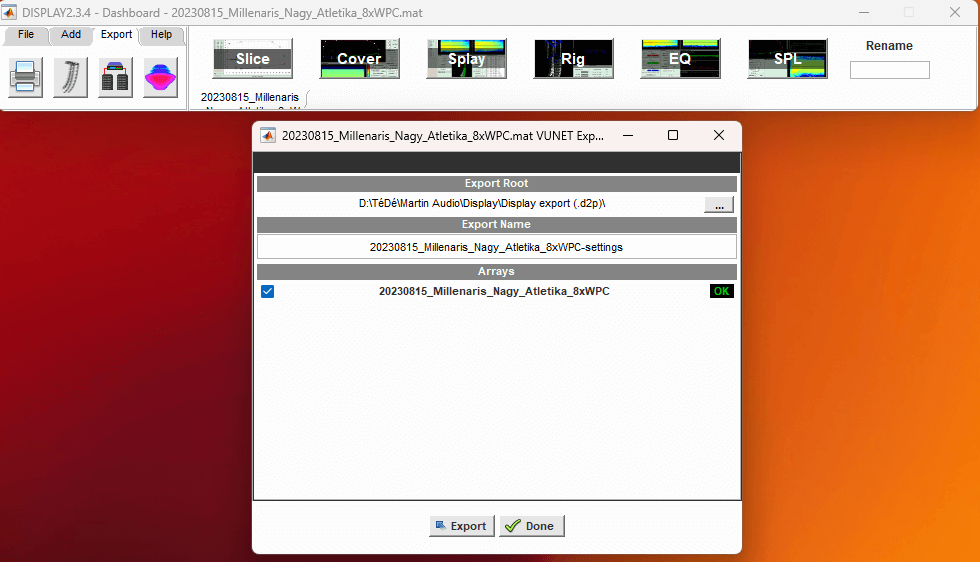
\includegraphics[width=\textwidth, keepaspectratio]{figures/display_wpc_7.png}
	\caption{Display 2.3.4 b1 exportáló kezelőfelülete (WPC)}\label{fig:display_wpc_7}
\end{figure}
%----------------------------------------------------------------------------
A fő hangrendszer megtervezése után a következő részegység aminek a tervét el kell készíteni, az a Delay hangrendszer.
A Delay hangrendszer a fő hangrendszerrel együtt fog működni, és a közönségtér hátsó-közép részétől kezdve fogja kiegészíteni azt.
Erre azért van szükség, mert a csarnokban a közönség ezen része olyan távolságra helyezkedik el, hogy
a WPC rendszer már nem tudja a megfelelő hangnyomás szintet egyenletesen biztosítani.
Ezt a feladatot a Wavefront Precision sorozatból a WPM típusú hangládák fogják ellátni, oldalanként 6-6 darab LineArray modullal.
Ez a láda egy két utas passzív hangrendszer, 2 darab 6.5"-os mély hangszóróval (LF) és 3 darab 1.4"-es magas hangszóróval (HF). 
Maximásan 130 dB hangnyomás szintet tud biztosítani, nagy előnye ennek a fajta rendszernek a súly-teljesítmény aránya, mivel egy
darab láda mindössze 14 kilogramm. \cite{WPMUSERGUIDE}
%----------------------------------------------------------------------------
\begin{figure}[H]
	\centering
	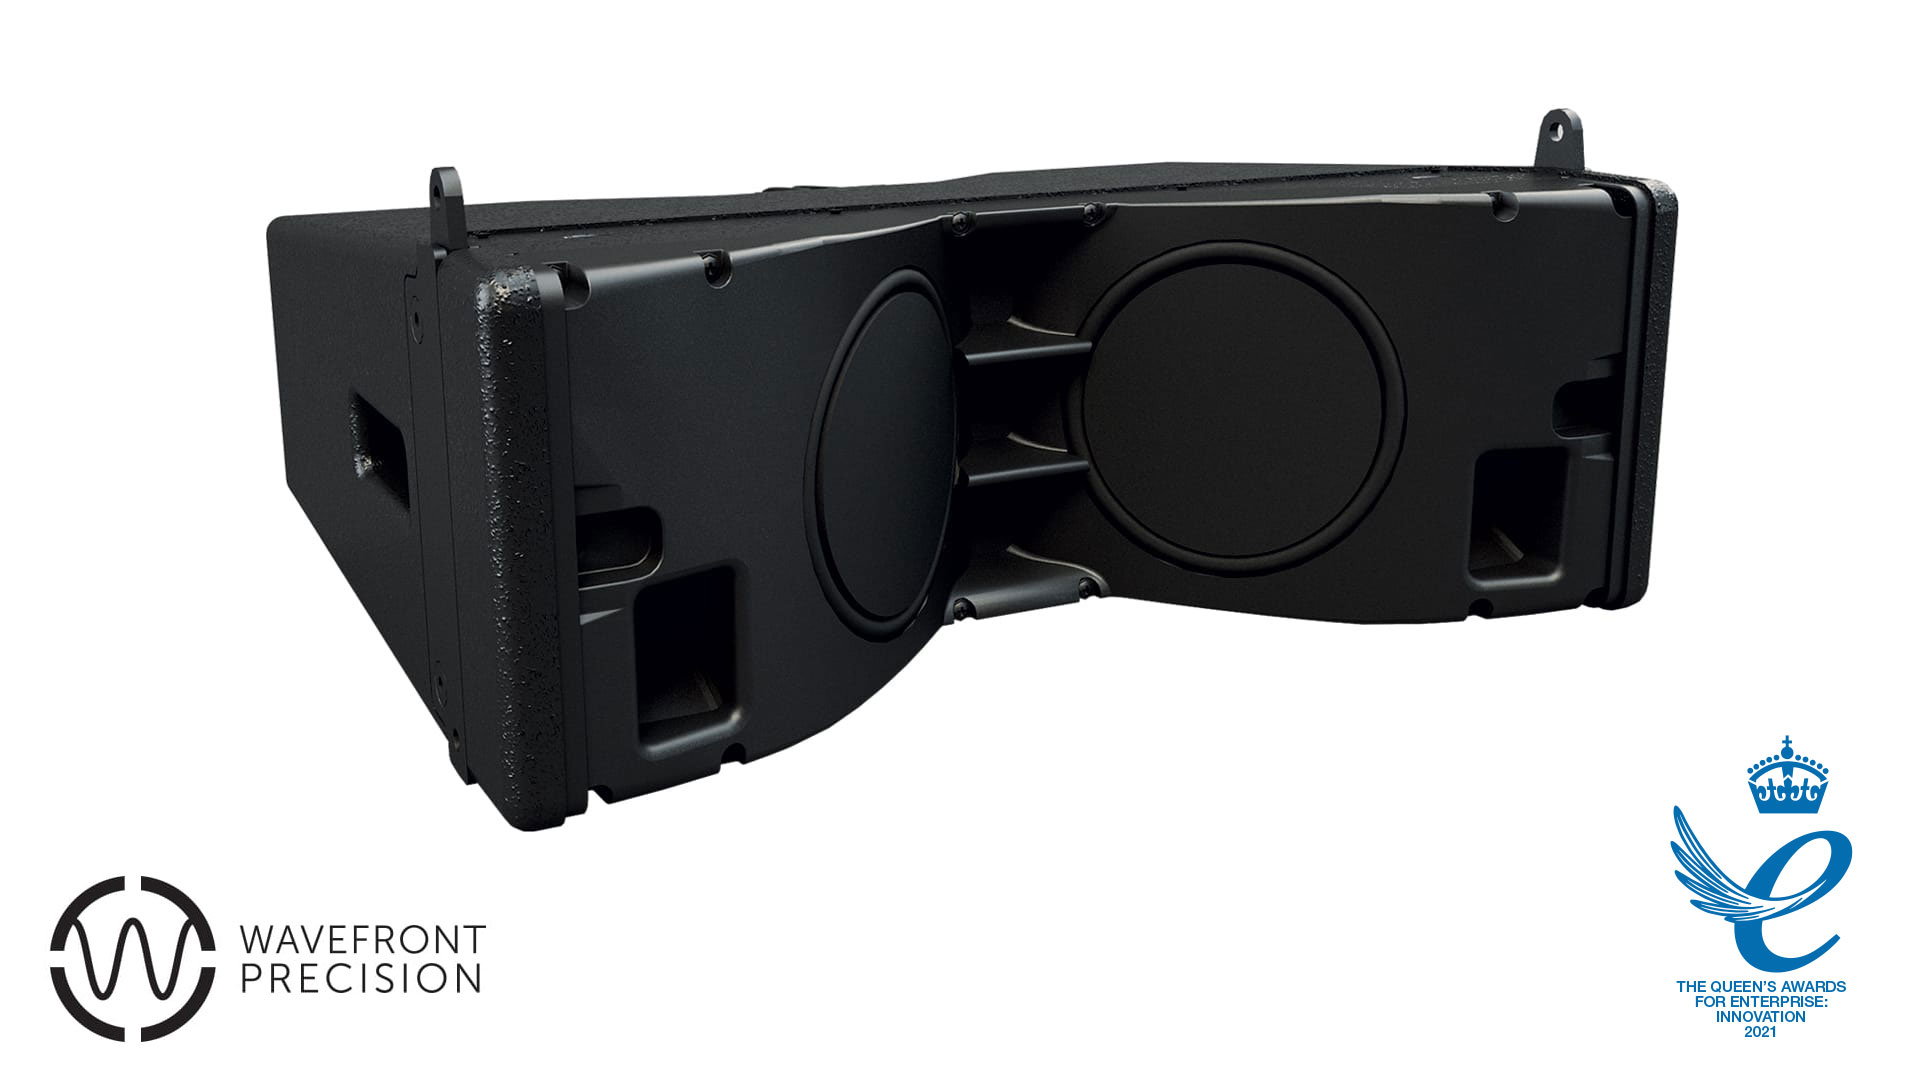
\includegraphics[width=80mm, keepaspectratio]{figures/wpm_front_view.jpg}
	\caption{Martin Audio WPM LineArray modul}\label{fig:wpm}
\end{figure}
%----------------------------------------------------------------------------
A tervezési fázisok nagy része megegyezik az előbbi rendszer tervezésével, ezért ezeket a részeket nem ismétlem meg.
A hangsúlyt a eltérésekre helyezem, és azokat fogom részletezni.
A fő különbség a \textit{``Cover''} kezelőfelületen történik, ahol a \textit{``Hard Avoid''} területet kell megjelölni.
Ezen a rajzon már radikálisan szükség van erre a funkcióra, mivel a közönség területén kívül eső területen beton nagy felületek találhatóak,
amelyek jelentős hangvisszaverődést okoznának. 
%----------------------------------------------------------------------------
%\begin{figure}[H]
%	\centering
%	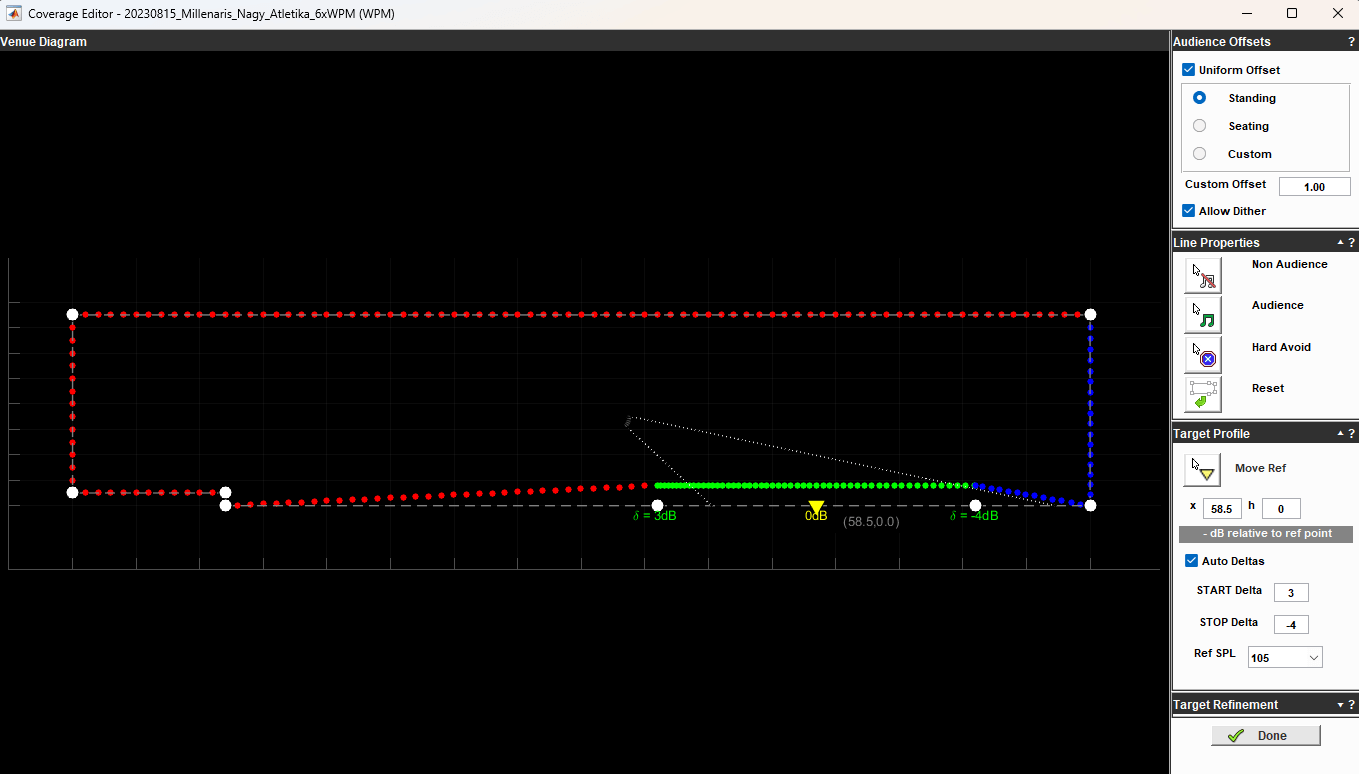
\includegraphics[width=\textwidth, keepaspectratio]{figures/display_wpm_1.png}
%	\caption{Display 2.3.4 b1 \textit{``Cover''} kezelőfelülete (WPM)}\label{fig:display_wpm_1}
%\end{figure}
%----------------------------------------------------------------------------
Ebből kifolyólag, szépen látható, hogy a program pontosan úgy optimalizálja a rendszert, hogy a \textit{``Hard Avoid''} területre, minél kevesebb
hangnyomás jusson.
Már a kék színnel jelölt terület első pár méterén radikálisan csökken a hangnyomás, és a rendszer a lehető legkevesebb energiát fordítja erre a területre.
A gyártó a WMP rendszert végfog csatornák szempontjából úgy tervezte, hogy a költség és a rugalmasság szempontjából akár négyesével is hajthatóak legyenek.
Ez persze nem jár kompromisszumok nélkül, a hangvisszaadás egyenletesebb lenne, ha egyesével hajtanánk a ládákat, de a jelenlegi rendszerben
hármasával fogom hajtani a ládákat, mivel ez a legköltséghatékonyabb megoldás, és végeredményben így is kielégítő hangvisszaadást fog produkálni mint 
kiegészítő egység. A WPM-eket tudjuk egyesével is hajtani, mivel rendelkezésünkre áll 2 db iK81 végfok.
%----------------------------------------------------------------------------
\begin{figure}[H]
	\centering
	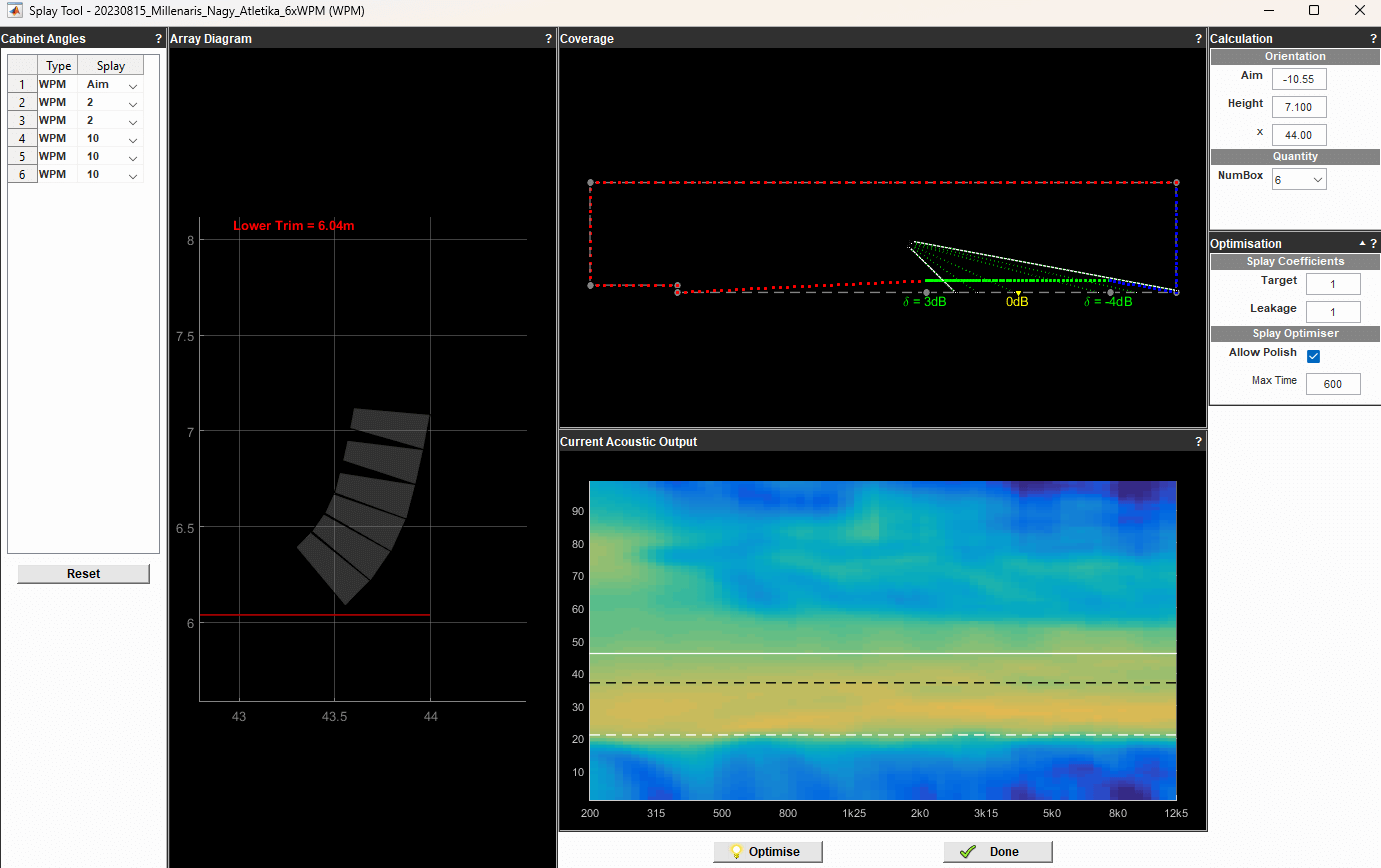
\includegraphics[width=\textwidth, keepaspectratio]{figures/display_wpm_2.png}
	\caption{Display 2.3.4 b1 \textit{``Splay''} kezelőfelülete (WPM)}\label{fig:display_wpm_2}
\end{figure}
%----------------------------------------------------------------------------
Az előbbiekben már tárgyalt exportáló felületen az összes többi optimalizációs lépést követően
mentjük az elkészített tervet a WPC rendszerhez hasonlóan.
%----------------------------------------------------------------------------
\subsubsection{Martin Audio VU-NET rendszer szoftver \cite{VUNETUSERGUIDE}}
%----------------------------------------------------------------------------
Első és legfontosabb feladatunk, hogy az összes végfoknak egyedi IP címet adjunk a hálózaton.
Enélkül a rendszerünk használhatatlan lesz, mivel a VU-NET szoftver nem fog tudni kommunikálni a végfokokkal.
Ezután győződjünk meg, hogy számítógépünk ugyan abban az alhálózatban és cím tartományban van mint a többi eszköz.
Miután már rendelkezünk az összes számunkra szükséges rendszer patch fájljával,
el tudjuk kezdeni felütni a végfokparkot amelyek a hangszórókat fogják hajtani.
Tehát a következő lépések a VU-NET szoftverben történnek a végfokok beállításával.
A VU-NET szoftver egy olyan alkalmazás, amely lehetővé teszi a Martin Audio hangrendszerek teljes körű vezérlését és monitorozását.
Jelen esetben az iK42 és iK81 típusú eszközöket fogjuk tudni kezelni.
Rendszerünk ha mindent összeszámolunk, akkor 8 darab iK42 és 2 darab iK81 végfokot fog tartalmazni.
Ebből 4 db iK42 a WPC LineArray rendszert, 2 db iK81 a WPM LineArrayt, 3 db iK42
az SX218 mélyládákat, és 1 db iK42 a FrontFill hangfalakat (XD12) fogja hajtani.
A Discover Devices gombra kattintva a szoftver megkeresi az összes végfokot a hálózaton, és megjeleníti azokat a
cím szerint növekvő sorrendben. Szinkronizáció után szabadon vezérelhetővé válnak az eszközök.
Egy kiválasztott eszközre jobb egérgombbal kattintva megjelenik egy menü, ahol az Open Preset Manager opcióra kattintva
betölthetjük az előre elkészített és gyári preseteket.
Az alábbi képen látható az a felület ahol bele kell tölteni a preseteket az egyes erősítőkbe külön-külön.
%----------------------------------------------------------------------------
\begin{figure}[H]
	\centering
	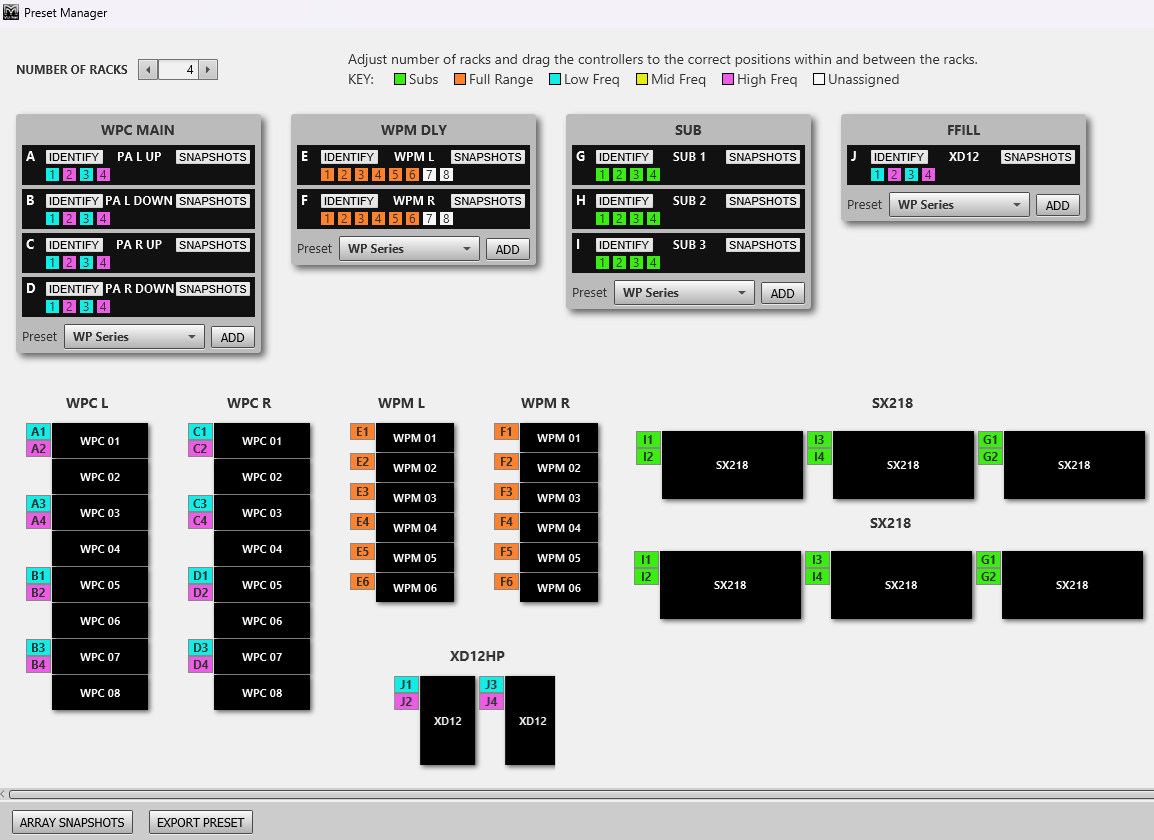
\includegraphics[width=\textwidth, keepaspectratio]{figures/vunet_systemdiagram_overall.png}
	\caption{VU-NET rendszer áttekintő diagram}\label{fig:vunet_systemdiagram_overall}
\end{figure}
%----------------------------------------------------------------------------
Így már szépen látható, hogy a rendszerünk hogyan fog kinézni, és melyik végfok melyik csatornán mit fog hajtani.
Ez kábelezés és rendszerstruktúra szempontjából is nagyon fontos információ, mivel kizárólag a megfelelő helyre
kötött hangládákkal fog megszólalni helyesen a rendszer. Ezen felül ha valamit rossz helyre kábelezünk le, tegyük fel egy
mélyládát hajtó végfokra egy Line Array modult, akkor a benne lévő hangszórók nagy valószínűséggel tönkremennek ha terhelés alá kerülnek.
Tehát fontos az precíz és átgondolt munkavégzés. A hibák elkerülése után is hasznos számunkra a rendszer áttekintő diagram,
mivel ha valami nem működik a rendszerben, akkor könnyen és gyorsan megtalálhatjuk a hibát, és azonosíthatjuk a hibás komponenst.
Miután sikeresen betöltöttük az összes presetet amire szükségünk van, be kell állítanunk, hogy az erősítők milyen forrásból
fognak jelet kapni. A következő lépésben a routing fülön be kell állítanunk, hogy az input csatorna Dante hálózatról fogja kapni a jelet.
Ez a beállítás a következőképpen néz ki:
%----------------------------------------------------------------------------
\begin{figure}[H]
	\centering
	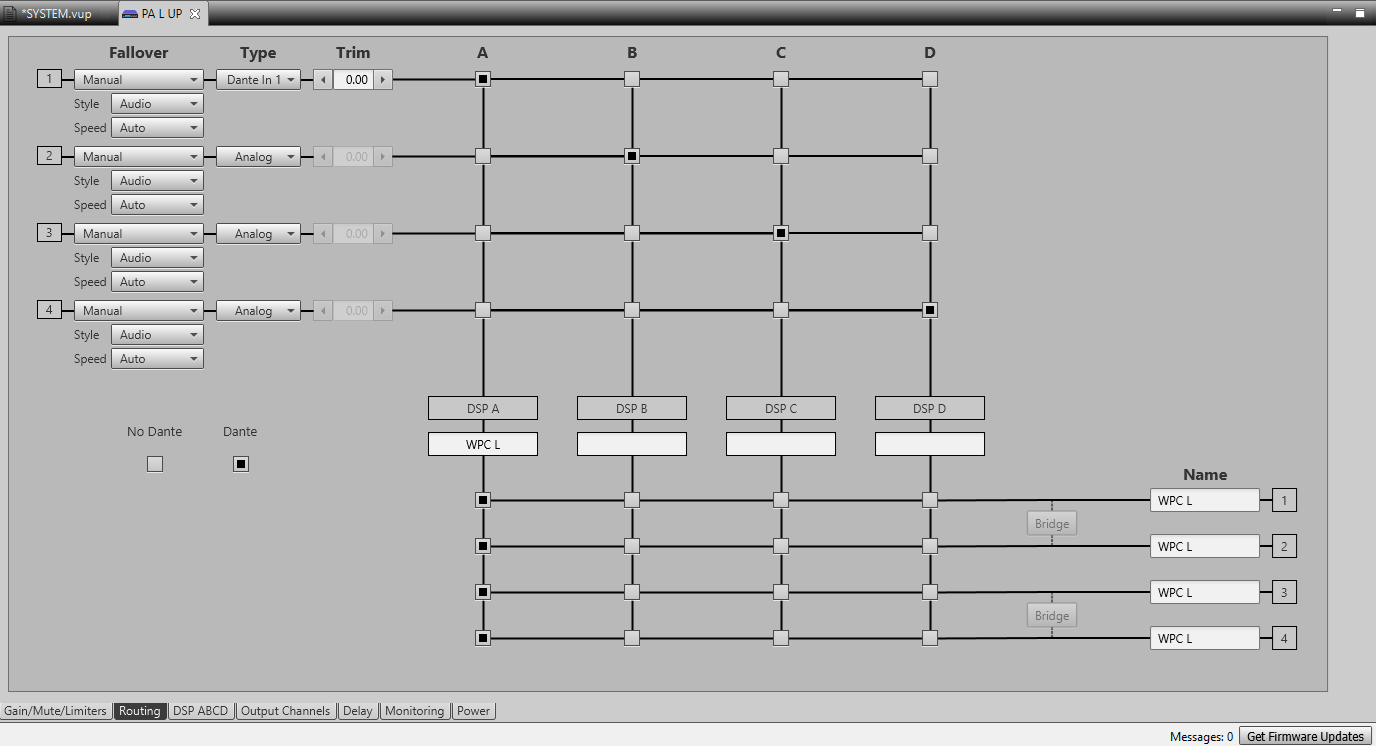
\includegraphics[width=\textwidth, keepaspectratio]{figures/vunet_routing_dante.png}
	\caption{VU-NET Dante routing}\label{fig:vunet_routing_dante}
\end{figure}
%----------------------------------------------------------------------------
Most, hogy a megfelelő alapbeállításokat elvégeztük, a rendszer készen áll arra, hogy zajjal, például
Pink Noise-al teszteljük. Ezalatt a rendszer minden egyes komponensét külön-külön lehallgatjuk, és ellenőrizzük,
hogy minden egyes hangszóró megfelelően működik-e. Ha rendellenességet észlelünk, akkor azonnal kikapcsoljuk a rendszert,
és megnézzük, hogy mi okozza a problémát. Ha a probléma nem oldható meg, akkor a rendszert nem szabad tovább használni,
és az adott komponenst cserélni kell. Ha minden rendben van, akkor a rendszer készen áll a további feladatokra, mivel
még koránt sem értünk a végére a folyamatnak. A programba a mérési és optimalizálási folyamat közben még sok beállítást kell
elvégezni, amelyekről a későbbiekben lesz szó.
%----------------------------------------------------------------------------
\subsection{Dante hálózat kialakítása és optimalizálása}
%----------------------------------------------------------------------------
\subsubsection{Dante Controller}
%---------------------------------------------------------------------------- 
% Hálózati mátrix
%----------------------------------------------------------------------------
Ezen a felületen tudjuk a hálózaton összekapcsolni a különböző hang vevőket és
adókat. Egy nagyobb rendszerben a konfigurálása rendkívül nagy odafigyelést és
precíziót igényel, pontosan tudnunk kell mit, hogyan és miért kötünk össze.
%----------------------------------------------------------------------------
% Eszköz nézet
%----------------------------------------------------------------------------
Mielőtt neki állnánk konfigurálni az adott eszközt, fontos eldöntenünk, hogy
milyen módban szeretnénk használni.
Lehetőségünk van két fő mód közül választani, a redundáns és a
váltott mód közül. A \textit{``redundant''} mód mint ahogy azt a neve is sugallja
redundáns kommunikációt valósít meg az eszközök között szoftveresen és
hardveresen egyaránt. Az összes Dante kártya a jelenlegi rendszerben gyári konfigurációban két RJ45-s
csatlakozóval rendelkezik. Jelen esetben ezt a módot választjuk az
üzembiztosság és a kritikus hibák minimalizálása miatt.
A másik lehetőség a \textit{``switched''} pedig eszközök láncolását
teszi egyszerűbbé. Amennyiben a redundancia nem elsődleges szempont számunkra, nem kell
minden egyes eszköz mögé switch, hanem a másodlagos RJ45 port direktbe köti
az arra csatlakoztatott eszközt az elsődleges hálózatra. Így gyorsabban és
költséghatékonyabban tudjuk kiépíteni a hálózatot, azonban a redundancia lehetősége megszűnik.
%----------------------------------------------------------------------------
\subsubsection{IP kiosztás}
%----------------------------------------------------------------------------
A rendszer képes automatikusan IP címeket osztani az egyes eszközöknek,
ezzel meggyorsítva a munkafolyamatot. Viszont ez nem bizonyul jó megoldásnak.
Egy fixen előre megtervezett rendszer praktikusabb és
üzembiztosabb megoldás, ha minden eszköznek manuálisan mi adjuk meg a címét a
hálózaton. A tervezett rendszerben minden egyes eszköznek fix IP címet adtam,
hogy könnyen és logikusan átlátható legyen az előbb említett előnyökön kívül.
A címeket egy online is elérhető Excel táblázatban tároltam, hogy amennyiben szükség van rá
bármikor könnyen elérhető legyen. Ez a táblázat a cégnél dolgozó összes munkatárs számára látható,
aki a rendszerrel foglalkozik. Így amennyiben új eszköz kerül a hálózatra, vagy egy eszköz IP címét
valamilyen okból meg kell változtatni, egyszerűen elérhető a szükséges naprakész információ.
A kiosztás logikája a következőképpen néz ki:
A Dante Primary hálózat a 192.168.1.X címeket használja, a Secondary hálózat
pedig a 192.168.2.X címeket. A két hálózat között nincsen semmilyen kapcsolat, és egymástól teljesen függetlenek hardveresen és szoftveresen is.
A Vu-Net vezérlés a 192.168.100.X címeket használja, és egy switchen keresztül üzemel a secondary hálózaton, viszont a két hálózat között nincsen
átfedés, az előbbiekben már említett módon függetlenek egymástól.
Az eszközök egyedi címei pedig az alábbi módon kerültek kiosztásra:
Vegyük példának a 192.168.1.111-es címet, a 111-ben az első számjegy arra utal, hogy egy végfokról van szó, minden végfok
1XX címet kap. A második számjegy az eszköz rack száma, a harmadik pedig az eszköz sorszáma a rackben felülről lefelé.
Tehát az előbbi cím a következőt jelenti számunkra: Az 1-es sorszámú végfokrackben lévő legfelső végfok.
A keverőpultok a címezés elején 1-től indulva 20-ig kapnak címeket. A stageboxok 30-tól 50-ig kapnak címeket.
Ezeken felül a háló legvégére vannak kiosztva a speciális eszközök melyek nem mindig vannak a rendszerben, de ha mégis
akkor azoknak is megvan a saját címük.
A háló 250-es címén helyezkedik el a Dante Audio szerver.

%----------------------------------------------------------------------------
\begin{figure}[H]
	\centering
	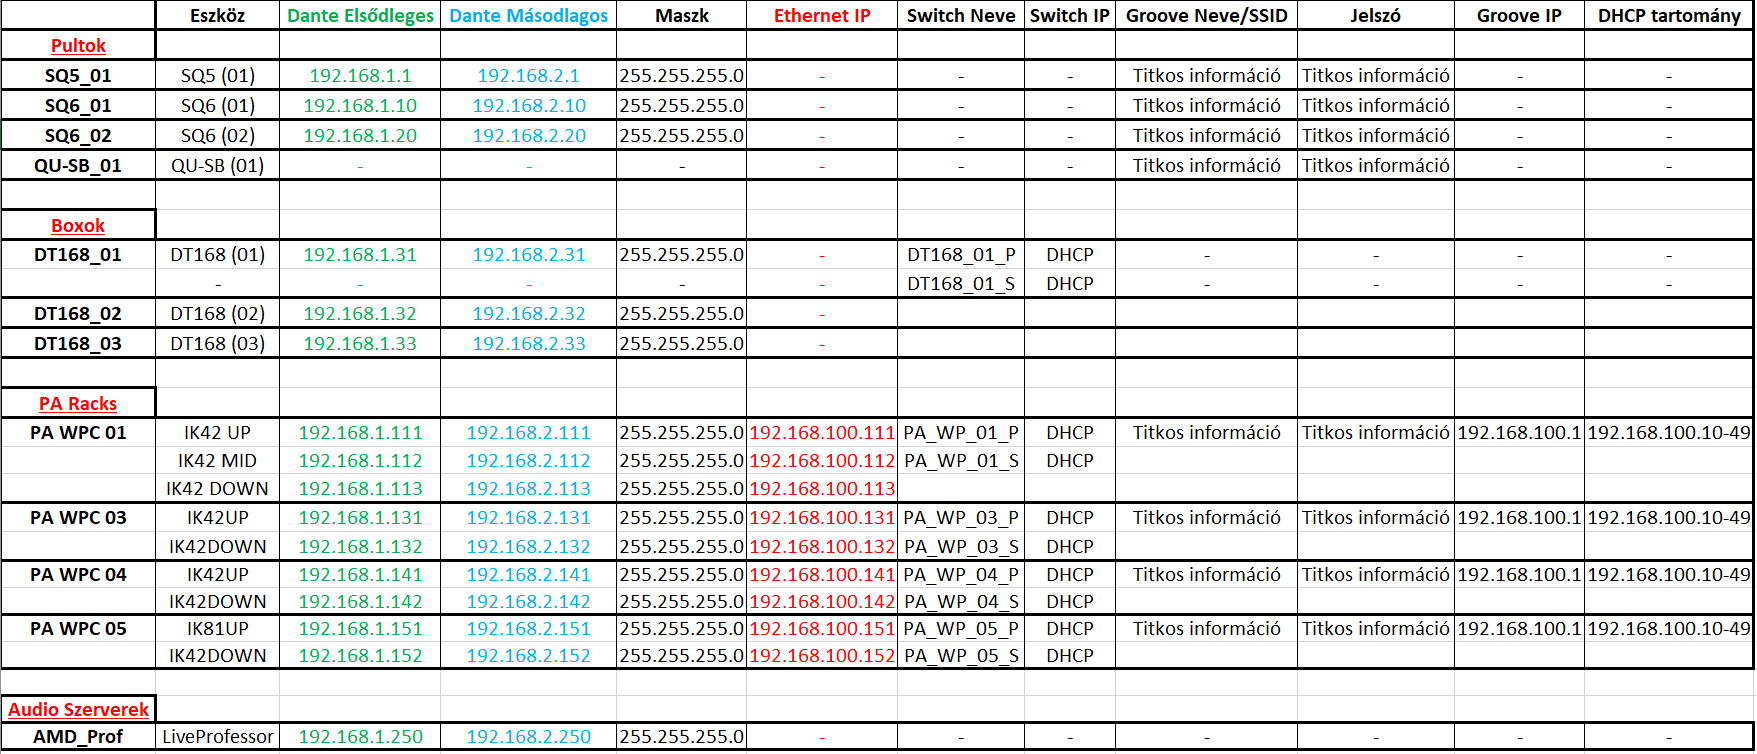
\includegraphics[width=\textwidth, keepaspectratio]{figures/dante_ips.png}
	\caption{Dante eszközök IP címei a hálózaton}\label{fig:dante_ips}
\end{figure}
%----------------------------------------------------------------------------
%----------------------------------------------------------------------------
% Órajel nézet és késleltetés
%----------------------------------------------------------------------------
Meg kell adnunk az audio hálózatunk master órajelét. Ehhez az órajelhez
szinkronizál a többi eszköz.
Az időszinkronizáció kulcsfontosságú élőzenei produkcióknál.
A mi esetünkben a keverőpult lesz a master órajel, ő fogja a hálózatot
vezérelni. A felületen egyszerűen bepipáljuk a \textit{``Preferred leader''} opciót
a keverőpult mellett, és a hálózat többi eszköze automatikusan ehhez az órajelhez szinkronizálódik.
Az órajelen kívül a késleltetési értékeket is be kell állítanunk. A default érték minden eszköznél jelen esetben
1 ms, mivel ennél az értéknél a legtöbb eszköz képes probléma nélkül működni. Ez az érték azonban
nem minden esetben optimális, ezért fontos, hogy minden eszköz késleltetését ellenőrizzük és beállítsuk.
Amennyiben problémákat, zavaró pattanásokat vagy hangkimaradásokat tapasztalunk, akkor a késleltetési értékeket
növelni kell mindaddig, amíg a probléma nem szűnik meg. Fontos megjegyezni, hogy a késleltetési értékek
növelésével egyre több és több időt vesz igénybe a jelek feldolgozása, előzenei produkcióknál ez kritikus.
A mi esetünkben mivel az útválasztók is kifejezetten csak erre a célra vannak használva és semmiféle más
adatforgalmat nem bonyolítanak, a 1 ms-os késleltetési érték csökkenthető is akár a felére is.
Rövid kábelhosszak esetén egyes eszközök között akár 0.25 ms-os késleltetési értéket is beállíthatunk amennyiben
hosszútávon nagy biztonsággal stabil a hálózat.
%----------------------------------------------------------------------------
\subsubsection{Dante rendszer monitorozása}
%----------------------------------------------------------------------------



%----------------------------------------------------------------------------
% Hálózati állapot nézet
%----------------------------------------------------------------------------



%----------------------------------------------------------------------------
% Események nézet
%----------------------------------------------------------------------------





%----------------------------------------------------------------------------
\subsection{Mélyláda rendszer}
%----------------------------------------------------------------------------
A mélyláda hangja hosszabb hullámhosszú, mint a többi komponensé, ezért az
optimális helymeghatározásuk és elhelyezésük kulcsfontosságú a megfelelő
hangzás érdekében. 
A rendszerben a Martin Audio SX218 típusú mélyládáit fogjuk használni.
Ezek a ládák dupla 18"-os mély hangszórókkal vannak felszerelve, 2000W AES és 8000W csúcsteljesítményre képesek, és
maximálisan 144 dB hangnyomás szintet tudnak biztosítani. \cite{SXSUBWOOFERUSERGUIDE}
Jelen esetben 12 darab ilyen láda fogja biztosítani a megfelelő mély tartományt a rendezvényen.
%----------------------------------------------------------------------------
\begin{figure}[H]
	\centering
	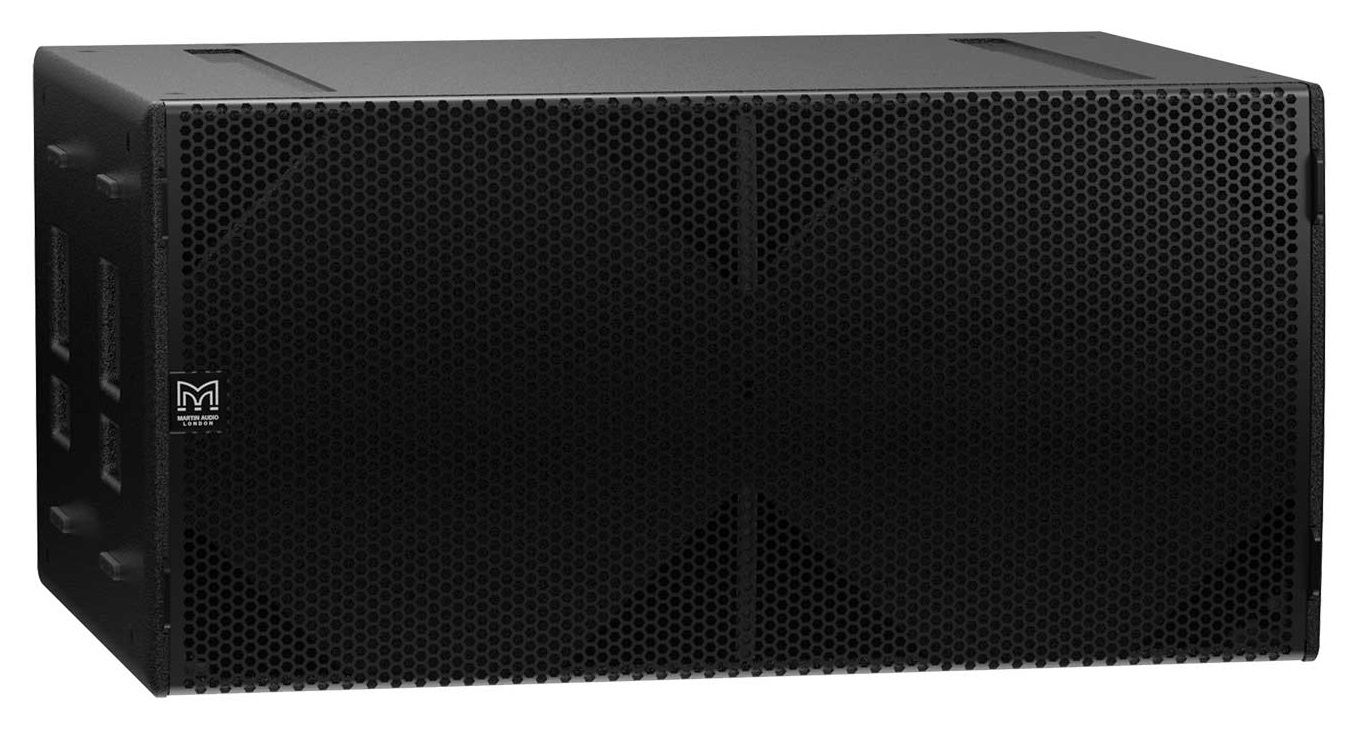
\includegraphics[width=80mm, keepaspectratio]{figures/sx218_front_view.jpg}
	\caption{Martin Audio SX218 mélyláda}\label{fig:sx218}
\end{figure}
%----------------------------------------------------------------------------
A \textit{``SUB''} tervezést egy általam készített Excel kalkulátor
segítségével végzem el. Ez a táblázat egyesíti a Martin Audio és Merlin van Veen által
készített kalkulátorokat (S.A.D), valamint kiegészítésre került további modulokkal és funkciókkal. \cite{MERLINVANVEEN} \cite{MARTINSUBCALCULATOR}
A egy EndFire konfigurációs mélyláda elrendezést terveztem. 
(Egy EndFire Pack = két láda egymás előtt adott távolságra és késleltetési értékkel) 
A táblázatba megadhatjuk, hogy éppen helyileg hol
van a rendezvény, és egy időjárás API segítségével megkapjuk az adott napra/napokra a
teljes időjárás előrejelzést. Majd ezekből egy adott időintervallumra átlagolva
megkapjuk az optimális értékeket a tervezéshez. 
A program kiszámolja, hogy milyen távolságra kell a ládákat helyezni egymástól előrefelé,
valamint mekkora \textit{``delay''} értéket kell alkalmazni. 
Majd az egyes EndFire Pack-ok egymáshoz képesti távolságot oldalirányban és azok
közötti delay értéket is megkapjuk. A \textit{``SUB array''}-t 63 Hz-re optimalizáltam, mivel
ez az a frekvenciatartomány, ahol a mélyláda rendszer a legtöbb energiát tudja leadni.
%----------------------------------------------------------------------------
\subsection{Allen \& Heath digitális keverőrendszer}
%----------------------------------------------------------------------------
A jelenlegi rendszer két keverőpultot fog tartalmazni, egyet a fő hangrendszerhez, és egyet a monitor rendszerhez.
Mindkét keverőpult Allen \& Heath SQ-6 típusú digitális keverőpult lesz.
A pultok 96 kHz-es mintavételezési frekvenciával operálnak és 48 csatornát képesek maximálisan kezelni, melyek közül 
24 csatornával rendelkezik fizikailag beépített mikrofon előerősítővel. A konzolokon található 16 programozható gomb,
25 fader melyek 6 rétegben helyezkednek el és a felhasználó személyre szabhatja őket a saját igényei szerint. 
Emellett 12 sztereó mix áll a rendelkezésünkre, melyeket szintén a felhasználó konfigurálhat saját igényei szerint.
A sztereóm mixek testreszabásával tudunk csoportokat is létrehozni.
A konzolokon 8 sztereó effekt motort is megtalálunk, ezekbe a virtuális effekt processzorokba a pultokon található ingyenes és fizetős 
pluginokat tudjuk betölteni. (amennyiben megvásároltuk a fizetős csomagokat, jelen rendszerben ezek nincsenek megvásárolva)
További előnye a platformnak, hogy egy 32x32 csatornás USB audio interfésszel rendelkezik, így a számítógéphez csatlakoztatva
egy nagy felbontású hangkártyaként is használhatjuk. \cite{AHSQ}
%----------------------------------------------------------------------------
\begin{figure}[H]
	\centering
	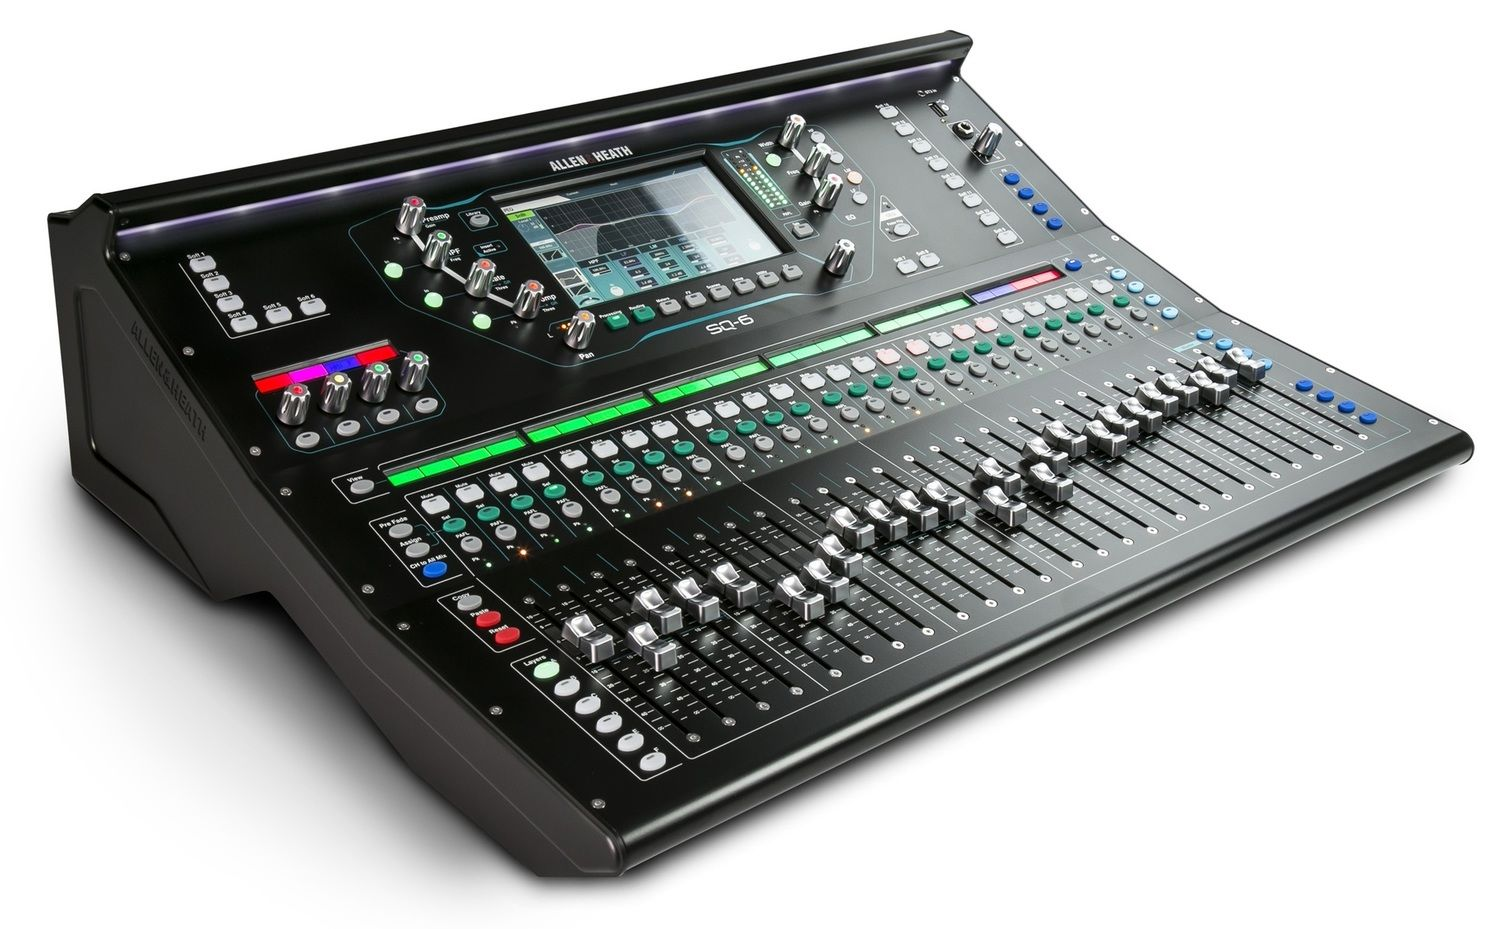
\includegraphics[width=80mm, keepaspectratio]{figures/sq6.jpg}
	\caption{Allen \& Heath SQ-6 digitális keverőpult}\label{fig:sq6}
\end{figure}
%----------------------------------------------------------------------------
Az I/O bővítőkártyák közül a rendszerben mindkét pultban megtalálható egy darab SQ Dante kártya ami 64x64 csatorna
kezelésére képes. Az A\&H SQ szériás pultjai csak egy darab I/O bővítőkártyát tudnak kezelni, de léteznek
olyan rendszerek mint például az Avantis és a DLive szériás pultok, amelyek több I/O bővítőkártyát is tudnak kezelni.
Jelen esetben ez teljes mértékben felesleges, mivel a rendszerben kizárólag a Dante protokollra támaszkodunk.
%----------------------------------------------------------------------------
\begin{figure}[H]
    \centering
    \begin{minipage}{0.45\textwidth}
        \centering
        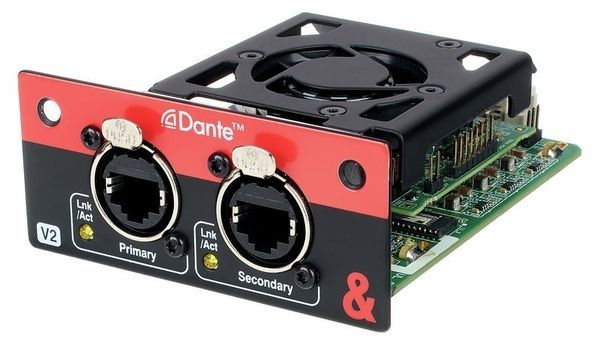
\includegraphics[width=60mm, keepaspectratio]{figures/sq_dante.jpg}
        \caption{A\&H SQ Dante kártya}\label{fig:sq_dante}
    \end{minipage}\hfill
    \begin{minipage}{0.45\textwidth}
        \centering
        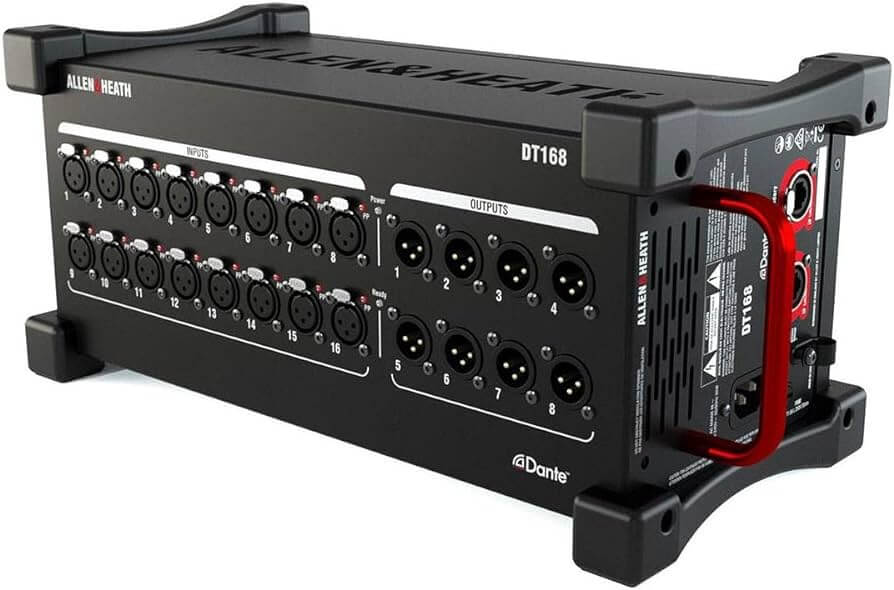
\includegraphics[width=60mm, keepaspectratio]{figures/dt168.jpg}
        \caption{A\&H DT168 Dante stagebox}\label{fig:dt168}
    \end{minipage}
\end{figure}

%----------------------------------------------------------------------------
\subsection{Dante audio szerver}
%----------------------------------------------------------------------------
Ez a kiegészítő szerver egység lehetővé teszi bármilyen alacsony késleltetéssel dolgozó VST3 plugin használatát a rendszerben elő környezetben.
Olyan komplex funkcionalitásokat is elérhetünk, amelyek a keverőpulton csak limitáltan, vagy egyáltalán nem elérhetőek.
Gondolva itt a dinamikus EQ használatára, különböző kompressziós technikákra (például Opto, Multiband Compressor), 
A legnagyobb előnye ennek a fajta megoldásnak, hogy költségek szempontjából egy magasabb kategóriás keverőpult rendszer sokkal drágább lenne,
valamint nem vagyunk korlátozva a keverőpult által biztosított funkcionalitásokkal, bármikor tudunk igényeink szerint újabb és újabb pluginokat
telepíteni a rendszerbe, amíg a számítógép hardveres erőforrásai ezt lehetővé teszik.
Az általam épített szerver egy AMD Ryzen 7950X processzorral és 32 GB DDR5 memóriával, és a Focusrite RedNet PCIe kártya veszi fel a harcot a
komplex hangfeldolgozási feladatokkal. Ezekre a hardverekre azért esett a választás, mert mivel a Dante kártya 128 csatornát tud kezelni, 
(az épített rendszer 64 csatornás, de a bővítés lehetősége fent áll) erős számítási kapacitásra van szükség, hogy a rendszer a beállított rendkívül alacsony
késleltetési értékek mellett is képes legyen késés nélkül a csatornák feldolgozására. Amennyiben nem sikerül a jelet a beállított időn belül
produkálni, furcsa zavaró pattogó hangokat hallhatunk, vagy rosszabb esetben hangkimaradás is előfordulhat. Ezért fontos a megfelelő hardveres
erőforrások biztosítása, és a pontos beállítások elvégzése.
A példában szereplő rendszer kifogástalanul képes elvégezni a feladatát, és a beállított 1 ms-os késleltetési értéket is képes folyamatosan tartani.
%----------------------------------------------------------------------------
\begin{figure}[H]
	\centering
	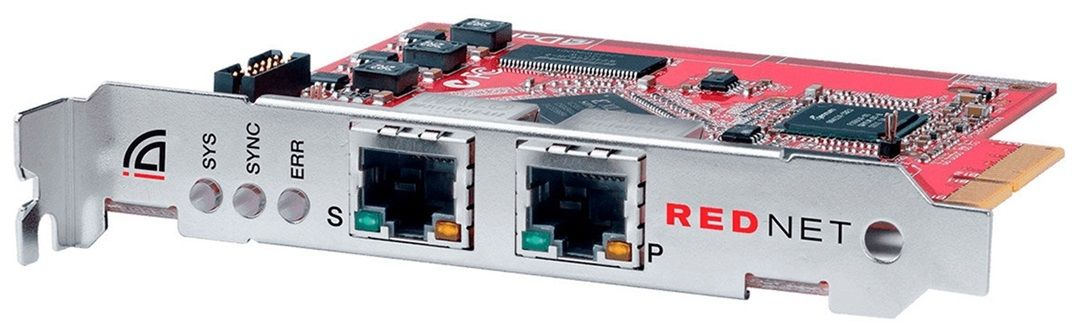
\includegraphics[width=67mm, keepaspectratio]{figures/rednet_pcie.jpg}
	\caption{Focusrite RedNet PCIe kártya}\label{fig:rednet_pcie}
\end{figure}
%----------------------------------------------------------------------------
Szoftveres oldalról a gépen egy speciális Windows 11 rendszer került telepítésre. A neve \textit{Ghost Spectre Windows 11 Superlite SE}, amely egy
teljesítmény és tárhely optimalizált Windows 11 verzió. A szakdolgozat írásakor elérhető legfrissebb stabil verzióját használtam fel, ami a
23H2-es 22631.3593 verziószámú.
A rendszerben csak a legszükségesebb alap szoftverek vannak telepítve, és a többi 
alkalmazás, amely nem szükséges a rendszer működéséhez, törölve lett. A lehető legkevesebb erőforrást használja, miközben egy stabil és megbízható
munkakörnyezetet biztosít. A frissítések automatikusan letiltásra kerültek, hogy a rendszer ne legyen kitéve a Windows frissítések által okozott
esetleges hibáknak, valamint a világhálóra való csatlakozás is letiltásra került. Kizárólag külső adathordozókról lehet adatokat átvinni a rendszerbe.
A számunkra szükséges drivereket és programokat kizárólag így tudjuk telepíteni a rendszerbe. 

%----------------------------------------------------------------------------


% !!! Képernyőfotó a szerverről !!! Leírás a pluginokról, singnal chain, hogy működik stb, plusz késés, mérések ilyesmi


%----------------------------------------------------------------------------
\subsection{A rendszer mérése}
%----------------------------------------------------------------------------
A rendszermérések elkészítésére a Rational Acoustics által fejlesztett Smaart nevű szoftvert fogom használni, mivel
az iparágban ez a legelterjedtebb és legmegbízhatóbb szoftver a mérések pontos elvégzésére.
A szoftver legújabb verzióját fogom használni, ami az írás pillanatában a 'Smaart Suite 9.4.1' verzió.
Első lépésben a számítógéphez csatlakoztatott hangkártyát kell konfigurálni, hogy el tudjunk kezdeni méréseket végezni.
Jelen esetben a hangkártya maga a keverőpult, aminek az USB interfésze egy 32x32-es kapcsolatra képes a számítógéppel.
A mérőmikrofon egy Behringer ECM8000 típusú mérőmikrofon lesz, ami XLR csatlakozóval kapcsolódik a keverőhöz, a mikrofon tápellátását
a keverőpult biztosítja 48V fantomtáppal. Annak érdekében, hogy a mérés működőképes legyen, a mikrofont a keverőpulton be kell szintezni, minden 
processzálást kikapcsolni. A mikrofon kimenetét utána Direct Out móddal el kell küldeni az USB interfészre, ahol a Smaart szoftver
fogja tudni a jelet feldolgozni. Ezen kívül egy másik bemenetre is szükség lesz a keverőpulton, ahol a Smaart szoftver a referencia jelet fogja
küldeni, ezt szintén Direct Out módban vissza kell küldeni a számítógépre.
Tehát a példa kedvéért még egyszer:
Local Input 1: Behringer ECM8000 mérőmikrofon, majd Direct Out Output USB 1-re.
USB Input 1: Smaart szoftver referencia jele, majd Direct Out Output USB 2-re.


Az első mérés amit végezni fogok a rendszeren a mélyláda rendszer mérése lesz.
Az EndFire konfigurációban elhelyezett mélyláda rendszer mérése során a cél az, hogy maximalizáljuk a hangnyomást a közönség távolabbi részein is,
miközben hátrafelé kioltást érünk el. Ezen felül fontos a rendszer nyitása is, ha túl keskeny sávban működik, akkor a középső területek
hangnyomása túl magas lesz, a szélső területeken pedig túl alacsony. Tehát fel van adva a lecke, hogy a rendszer a lehetőségekhez mérten
egyenletes hangnyomást biztosítson a teljes területen.
Fontos, hogy a mérési környezet a lehetőségekhez mérten minél csendesebb legyen, valamint
ne legyenek olyan tárgyak a nézőtéren, amelyek a rendszer elő működése közben
nem lesznek jelen és mérés közben a mért hangot visszaverik. Ezzel minimalizálhatjuk a
hibákat és a mérések pontatlanságát, valamint a mérés reprezentatívabb lesz.
%----------------------------------------------------------------------------
% SUB - TOP Align
%----------------------------------------------------------------------------
Mivel a mélyláda rendszer és a Main PA fizikai elhelyezkedésük miatt (A Main PA riggelve van, míg a mélyládák a földön helyezkednek el)
egy adott távolságra vannak egymástól, fontos, hogy a két rendszer fázishelyes és időhelyes legyen.
Amennyiben a rendszer fázishelytelen, a rendszer elemei egymás ellen dolgoznak, kioltást okozva, és ezzel csökkentve a hangnyomást.
Ezenkívül hiába van fázisban a rendszer, fontos, hogy a két rendszer időben is helyes legyen. Előfordulhat, hogy fázisban vagyunk de 180 fokkal el vagyunk tolva
az egyik irányba, így a mélyek vagy késnek vagy előbb érnek a hallgatóhoz ezzel rongálva a hangképet.
Aggodalomra azonban nincs ok, mivel megfelelő szakértelemmel és a megfelelő mérési eszközökkel ezek a problémák orvosolhatóak, ezzel biztosítva
a kiváló hangminőséget a rendezvényen.
Az alábbiakban a mérési eredmények láthatóak.
Fontos megjegyezni, hogy a mérési eredmények csak a mérés helyszínén érvényesek, és a mérési körülményektől függően változhatnak.
A reflexiók és a mérési bizonytalanság mennyisége infidecimális a mérési eredményben.
Az ábrán a következőket láthatjuk különböző színekkel jelölve:
- A kék szín a teljes rendszer viselkedése mérés nélkül.
- A zöld szín a teljes rendszer viselkedése mérés után.
- A magenta szín csak a main PA rendszer viselkedése.

%----------------------------------------------------------------------------
\begin{figure}[H]
	\centering
	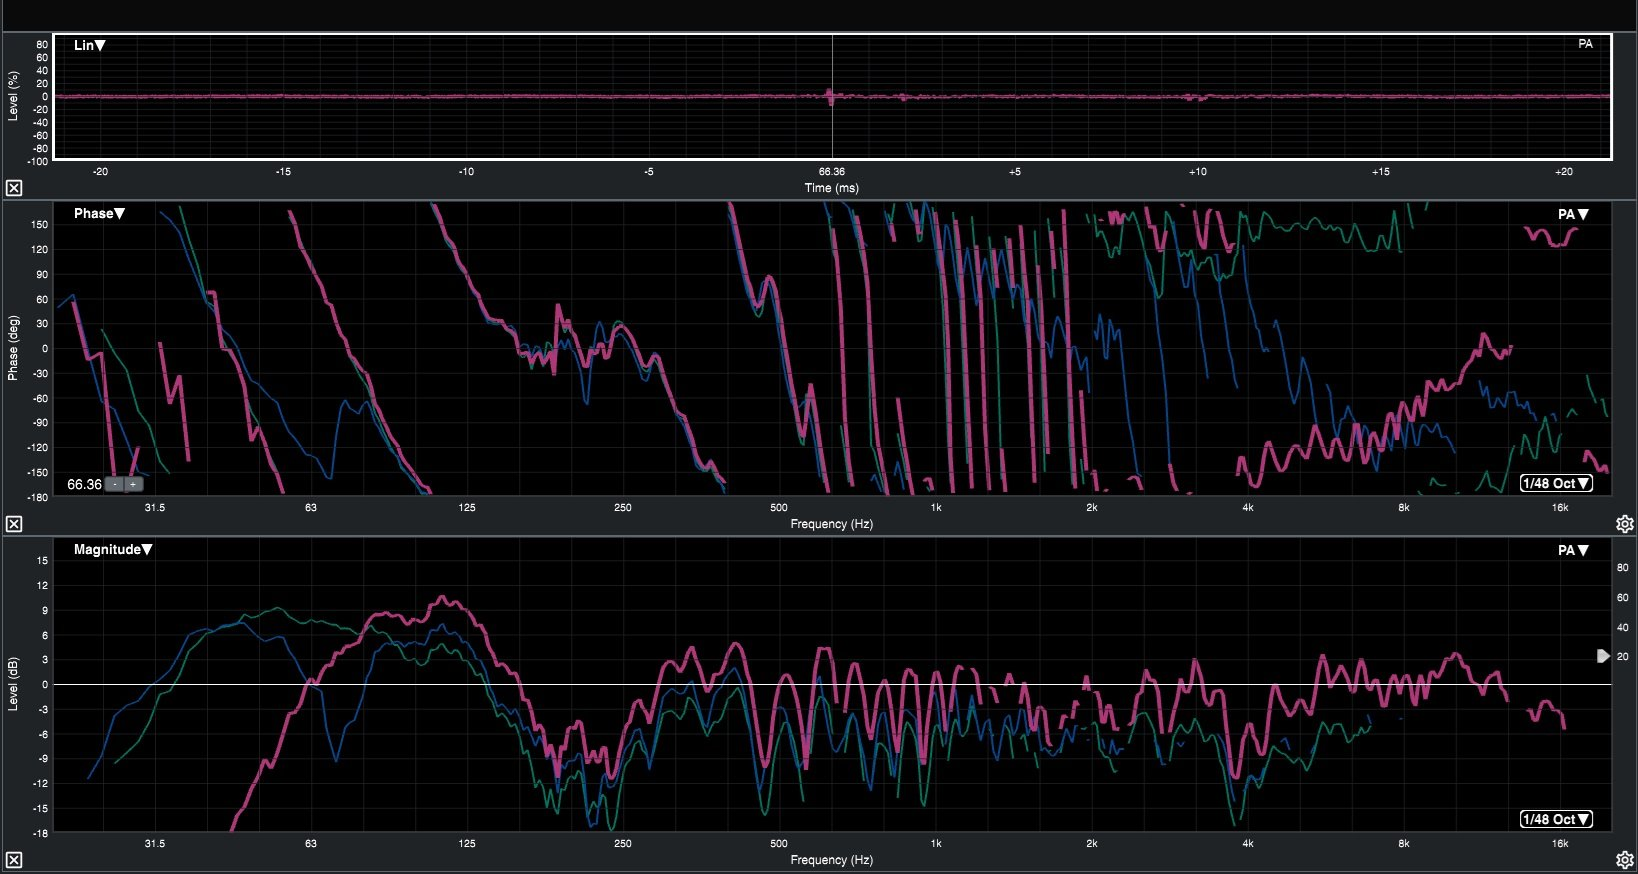
\includegraphics[width=\textwidth, keepaspectratio]{figures/smaart_sub_top.jpg}
	\caption{SUB - TOP mérések}\label{fig:smaart_sub_top}
\end{figure}
%----------------------------------------------------------------------------
Az ábrán egyértelműen látható, hogy a rendszer mérése után a hangnyomás szintje jelentősen nőtt, a crossover frekvencia környékén
57-87 Hz között. A kék mérésnél egy óriási beesést láthatunk 70 Hz-nél, ami azt jelzi számunkra, hogy a rendszer nincs fázisban és időben.
A korrekt időértékek beállítása után a zöld színű mérésnél egyértelműen látható, hogy a hangnyomás szintje jelentősen nőtt, és a 70 Hz-es
beesés teljes mértékben eltűnt, sőt a hangnyomás szintje a crossover frekvencia környékén jelentősen nőtt. Ez azt jelzi számunkra, hogy a rendszer
fázishelyes és időben is helyes már, készen áll a produkcióra.
%----------------------------------------------------------------------------
% FrontFill - TOP Align
%----------------------------------------------------------------------------










%----------------------------------------------------------------------------
\subsection{A rendszer monitorozása}
%----------------------------------------------------------------------------
Az időzítési értékek megfelelő beállítása után a rendszer hangnyomásának monitorozása a fontos.
A rendszer monitorozására a Smaart szoftverben található SPL monitor funkciót fogom használni.
Ehhez szükséges egy kalibrált mikrofon, amelynek a kalibrációs értékeit a Smaart szoftverben be kell állítani. 
Ez általában egy 94 dB-es referencia hangnyomás szintet jelent 1 kHz-en, melyet egy mikrofon kalibrációs eszközzel tudunk elvégezni ami képes pontosan kiadni ezt a hangnyomás szintet.
Így a mérési értékek pontosak lesznek, és a rendszer hangnyomás szintjét valósan tudjuk mérni.
Többféle módszerrel lehet a hangnyomás szintet monitorozni, jelen esetben hármat választottam ki:
- dB SPL C Slow => A frekvencia súlyozott hangnyomás szintet mutatja, a mikrofon érzékenységéhez igazítva.
- dB SPL A Slow => A frekvencia súlyozott hangnyomás szintet mutatja, az emberi hallás érzékenységéhez igazítva.
- dB Leq 1 => A hangnyomás szint átlagértékét mutatja 1 perces időtartamra.

%----------------------------------------------------------------------------
\begin{figure}[H]
	\centering
	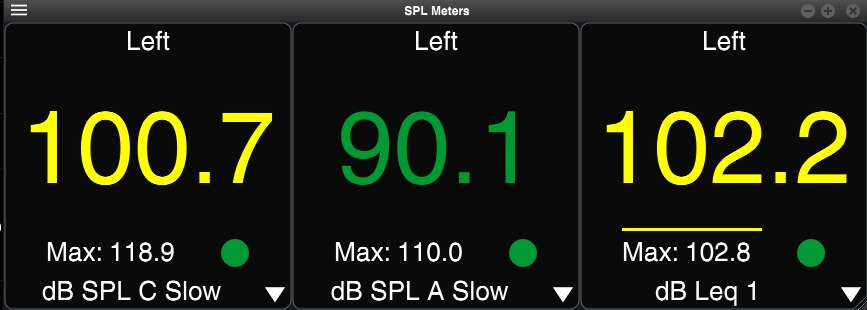
\includegraphics[width=100mm, keepaspectratio]{figures/smaart_spl_meter.jpg}
	\caption{SPL monitorozás a produkciók közben}\label{fig:smaart_spl_meter}
\end{figure}
%----------------------------------------------------------------------------